\documentclass[10pt,pdf,hyperref={unicode}]{beamer}


\usepackage[T2A]{fontenc}
\usepackage[utf8x]{inputenc}
\usepackage[english,russian]{babel}

\usepackage{amssymb,amsmath}

\usetheme[numbers, totalnumbers, minimal, nologo]{Statmod}
%\useoutertheme{dove}
\usecolortheme{dove}
%\usecolortheme[named=Brown]{structure} 
%\usecolortheme[RGB={205,173,0}]{structure} 


\usepackage{caption}
\usepackage{tikz}
\usepackage{pgfplots}
\usepackage{listings}

\usetikzlibrary{dsp,chains}
\usepackage{tikz-timing}

%\setbeamerfont{frametitle}{family=\rmfamily,series=\bfseries,size={\fontsize{12}{14}}}
\setbeamerfont{frametitle}{size={\fontsize{12}{14}}}

\defbeamertemplate*{title page}{customized}[1][]
{
  \vbox{}
  \vfill
  \begingroup
    \centering
    \begin{beamercolorbox}[sep=8pt,center,#1]{institute}
      \usebeamerfont{institute}\insertinstitute
    \end{beamercolorbox}
    \begin{beamercolorbox}[sep=25pt,center,#1]{title}
      \usebeamerfont{title}\inserttitle\par%
      \ifx\insertsubtitle\@empty%
      \else%
        \vskip0.25em%
        {\usebeamerfont{subtitle}\usebeamercolor[fg]{subtitle}\insertsubtitle\par}%
      \fi%     
    \end{beamercolorbox}%
    \vskip1em\par
    \begin{beamercolorbox}[sep=20pt,left,#1]{author}
      \usebeamerfont{author}\insertauthor
      
    \end{beamercolorbox}

    \begin{beamercolorbox}[sep=8pt,center,#1]{date}
      \usebeamerfont{date}\insertdate
    \end{beamercolorbox}\vskip0.5em
    {\usebeamercolor[fg]{titlegraphic}\inserttitlegraphic\par}
  \endgroup
  \vfill
}


\graphicspath{{images/}}

%\usefonttheme[onlymath]{serif}
\title[\theme]{Методы повышения качества обслуживания на основе потоковых агентов на стыке мобильных и стационарных сетей}

\author[Кобрин А. В.]{Аспирант: \ \ \ \ \ \ \ \ \ \ \ \ \ \ \ \ \ \ \ \ \ \ \ \ \
 \ \ \ \ \ \ Научный руководитель: \\Кобрин А. В. \ \ \ \ \ \ \ \ \ \ \ \ \ \ \ \ \ \ \ \ \ \ \ \ \
 \ д.т.н., проф. Поповский В.В.}
\institute[ХНУРЭ]{Харьковский Национальный Университет Радиоэлектроники}
\date{Харьков 2013}
\begin{document}



% титульная стр
\begin{frame}
\titlepage
\end{frame}
 
 \section{Архитектура сети NGN}

\begin{frame}
\frametitle{Архитектура сети NGN}
\begin{columns}[T]
\begin{column}{0.45\textwidth}
\begin{exampleblock}
{Уровни архитектуры сети NGN:}
\begin{itemize}
 \item Уровень управления услугами;
 \item Уровень сетевого контроля и управления;
 \item Транспортный уровень;
 \item Уровень доступа;
 \item Уровень терминального оборудования.
\end{itemize}
\end{exampleblock}
\end{column}
\begin{column}{0.5\textwidth}
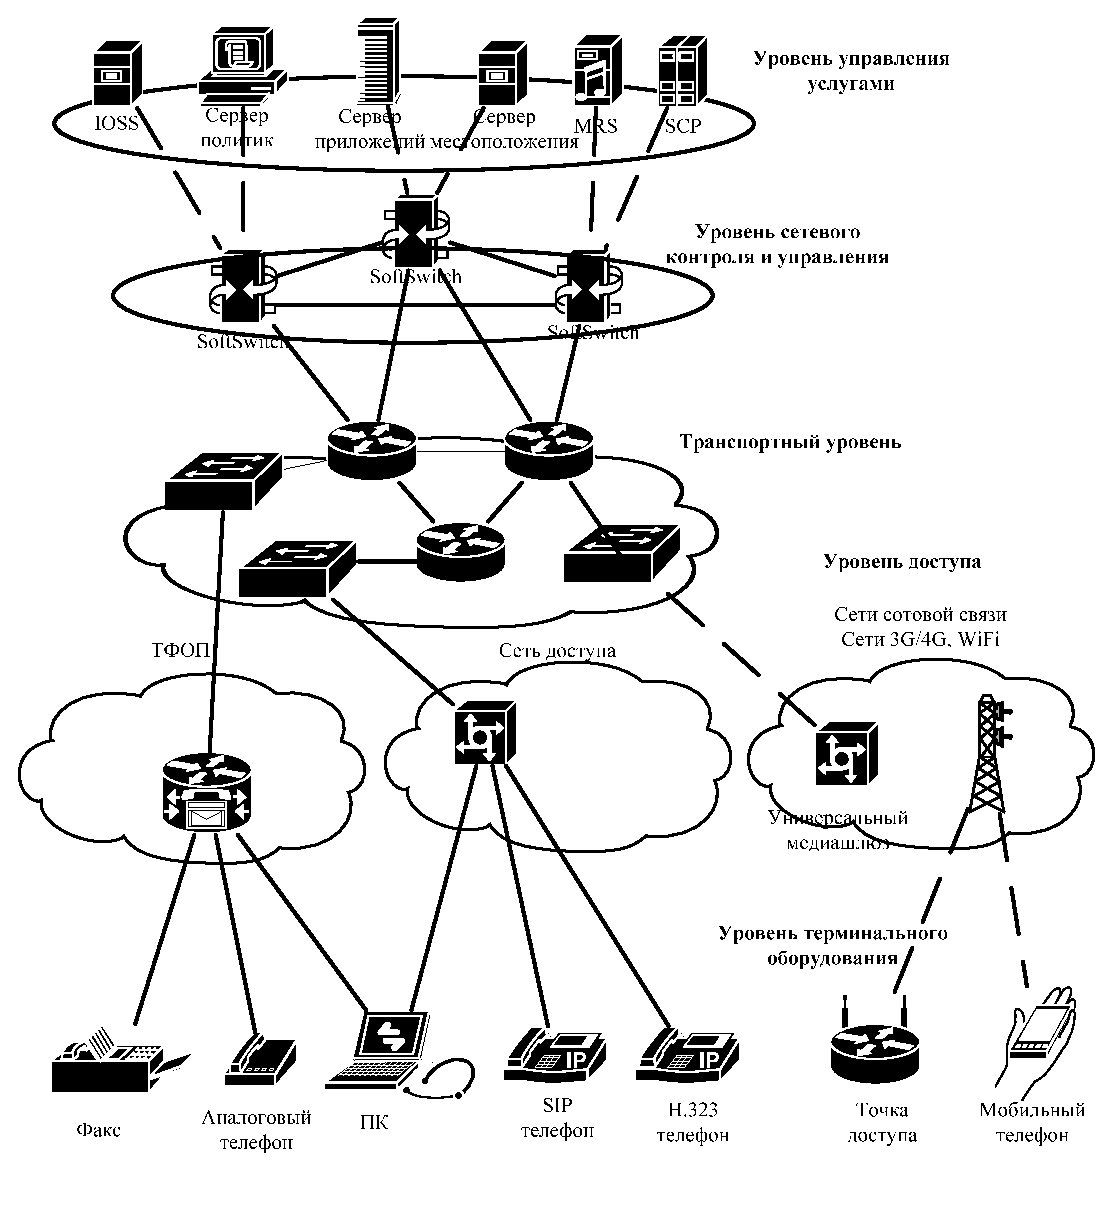
\includegraphics[width=\columnwidth]{ngn.eps}
\end{column}
\end{columns}
\end{frame}
 
 

 
\section{Цель и задача исследования}

\begin{frame}
\frametitle{Цель и задачи исследования}
{\footnotesize
\textbf{Цель и задача исследования} состоит в повышении качества обслуживания в гибридных сетях, содержащих мобильную и стационарную компоненту.

\textbf{Объект исследования:} процесс передачи трафика реального времени через гибридные сети.

\textbf{Предмет исследования:} метод повышения качества обслуживания на основе потоковых агентов на стыке мобильных и стацонарных сетей.

\textbf{Научная задача} состоит в повышении качества обслуживания в гибридных сетях, содержащих мобильную и стационарную компоненту.

\textbf{Частные задачи исследования:}
}
{\scriptsize
\begin{enumerate}
  \item Провести анализ статистических характеристик джиттера в стационарных и беспроводных сетях.
  \item Определить основные причины формирования джиттера.
  \item Определить статистические характеристики нестационарности джиттера и произвести классификацию нестационарных явлений задержки.
  \item Обосновать и разработать математическую модель джиттера, позволяющую отображать динамику нестационарных изменений состояний сетевой задержки.
  \item Разработать алгоритмы стохастической оценки параметров джиттера и управления с целью его минимизации.
  \item Разработать практические предложения по выбору параметров и мест установки потокового агента минимизации джиттера на границе стационарной и мобильной сети.
\end{enumerate}
}

\end{frame}
 
\section{Научная новизна полученных результатов}

\begin{frame}
\frametitle{Научная новизна полученных результатов}
{\small
\begin{enumerate}
  \item Получены более общие результаты анализа состояния составных каналов связи, включая мобильную и стационарную компоненту, выявлены причины возникновения нестационарностей и большого разброса параметров джиттера.
  Проанализированы механизмы формирования джиттера в гибридных сетях, получены статистические данные характеристик джиттера.
  \item Разработана более общая, по сравнению с известными, адекватная нестационарная математическая модель задержки прибытия пакетов,
  позволяющая учитывать засоренность представления наблюдаемого процесса случайными выбросами и скачками.
  \item 
  Разработан новый адаптивный метод компенсации джиттера на базе робастных процедур инвариантных к распределению вероятностей процесса задержки.
  \item 
  Разработаны новые рекомендации по применению буфера компенсации джиттера в сетях LTE на основе потоковых агентов, устанавливаемых на границе проводной и беспроводной сети.
\end{enumerate}
}
\end{frame}





\section{Первый научный результат}

\begin{frame}
\frametitle{Первый научный результат}

{\Large В результате анализа состояния составных каналов связи, включая мобильную и стационарную компоненту, выявлены причины возникновения нестационарностей и большого разброса параметров джиттера.
  Проанализированы механизмы формирования джиттера в гибридных сетях, получены статистические данные характеристик джиттера.}

\end{frame}






\section{Градация типов джиттера}
\begin{frame}
\frametitle{Градация типов джиттера}
\begin{columns}[T]
\begin{column}{0.35\textwidth}
{\small
\begin{exampleblock}
{Основные типы джиттера:}
\begin{enumerate}
 \item Постоянный джиттер;
 \item Джиттер содержащий выбросы задержки;
 \item Джиттер содержащий скачки задержки.
 \item Смешанный джиттер содержащий выбросы и скачки задержки.
\end{enumerate}
}
\end{exampleblock}
\end{column}
\begin{column}{0.65\textwidth}
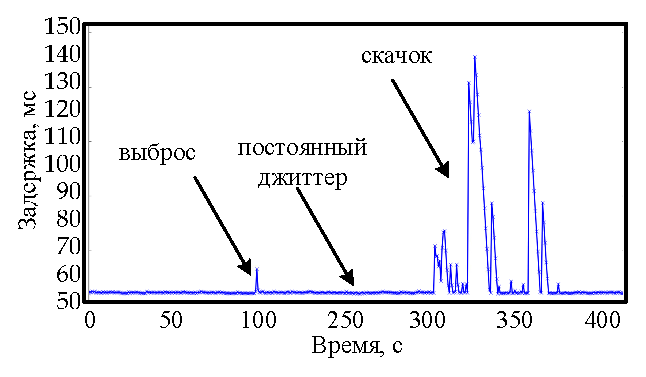
\includegraphics[width=\columnwidth]{3typeJitter.eps}
\end{column}
\end{columns}
\end{frame}






\section{Причины возникновения джиттера}



\begin{frame}
\frametitle{Причины возникновения джиттера}
{\footnotesize
\begin{exampleblock}
{Причины возникновения джиттера характерные для стационарных сетей:}
\begin{itemize}
\item Пакетное планирование на стороне отправителя (тип 1);
\item Перегрузка в локальной сети (тип 2);
\item Перегрузки в канале доступа (тип 3);
\item Распределение нагрузки между несколькими линиями доступа или сервис-провайдерами (тип 1);
\item Распределение нагрузки между несколькими маршрутами(тип 1);
\item Неравномерное внутреннее разделение нагрузки в маршрутизаторах (тип 1);
\item Влияние высокоприоритетного служебного трафика на менее приоритетный (тип 2).
\end{itemize}
\end{exampleblock}

\begin{exampleblock}
{Причины возникновения джиттера характерные для беспроводных сетей:}
\begin{itemize}
\item Хэндовер (тип 2);
\item Изменение расстояния между абонентом и базовой станцией (перемешение абонента) (тип 4);
\item Внутрисистемные и внесистемные помехи (тип 4);
\item Замирания в канале (тип 4).
\end{itemize}
\end{exampleblock}
}
\end{frame}







\section{Обзор архитектуры имитационной модели сети LTE в сетевом симуляторе NS3}


\begin{frame}
\frametitle{Обзор архитектуры имитационной модели сети LTE в сетевом симуляторе NS3}
\begin{figure} [h]
  \center
\includegraphics [width=0.95\textwidth] {LTEEPC.eps}
\end{figure}



\end{frame}



\section{Моделирование причин возникновения нестационарного джиттера в сети LTE}
\begin{frame}
\frametitle{Моделирование причин возникновения нестационарного джиттера в сети LTE}
\begin{figure} [h]
  \center
\includegraphics [width=0.80\textwidth] {hand-eps-converted-to.pdf}
\caption*{Изменение задержки прибытия пакетов при хэндовере между базовыми станциями}
\end{figure}
\end{frame}


\section{Моделирование причин возникновения нестационарного джиттера в сети LTE}
\begin{figure} [!h]
{\fontscript\begin{footnotesize}
\begin{minipage}[h]{0.47\linewidth}
\center
\includegraphics[width=1\linewidth]{Sinr_dist.eps} а) \\
\end{minipage}
\hfill
\begin{minipage}[h]{0.47\linewidth}
\center
\includegraphics[width=1\linewidth]{mcs_dist.eps} б) \\
\end{minipage}
\vfill
\begin{minipage}[h]{0.47\linewidth}
\center
\includegraphics[width=1\linewidth]{tb_dist.eps} в) \\
\end{minipage}
\hfill
\begin{minipage}[h]{0.47\linewidth}
\center
\includegraphics[width=1\linewidth]{speed_dist.eps} г) \\

\end{minipage}

\end{footnotesize}
\caption*{Зависимость а) SINR б) MCS в) размера TBS г) скорости передачи нисходящего канала передачи от расстояния между абонентом и базовой станцией}
\label{img:dist}
\end{figure}
\end{frame}





\section{Моделирование причин возникновения нестационарного джиттера в сети LTE}

\begin{frame}
\begin{columns}[T]
\begin{column}{0.5\textwidth}

\includegraphics[width=1\linewidth]{intervsSdj.png}
{\scriptsize \\Зависимость джиттера от расстояния до источника внутрисистемной помехи}

\end{column}

\begin{column}{0.5\textwidth}

\includegraphics[width=1\linewidth]{intervsSdr.png}

{\scriptsize \\Зависимость пакетных потерь от расстояния до источника внутрисистемной помехи}

\end{column}
\end{columns}
\end{frame}











\section{Моделирование причин возникновения нестационарного джиттера в сети LTE}
\begin{frame}
\begin{scriptsize}
\pgfplotsset{width=10cm, height=3.5cm, compat=newest}
\begin{figure} [!bth]
\begin{scriptsize}
\begin{minipage}[h]{0.95\linewidth}
  \center
\begin{tikzpicture}
\pgfkeys{/pgfplots/legend pos=north west}
\begin{axis}[
mark options={scale=0.7},
legend cell align=left,
%cycle list name=mark list,
cycle list name=linestyles*,
xlabel=Расстояние между абонентом и базовой станцией (м),
ylabel=Задержка (с),
]
\addplot coordinates {
(500,0.04)
(0,0.022)};
\addplot coordinates {
(500,0.053)
(0,0.022)};
\addplot coordinates {
(500,0.035)
(0,0.022)};
\legend{EVA, ETU, EPA}
\end{axis}
\end{tikzpicture}
%\caption{Зависимость задержки пакетов от расстояния между абонентом и базовой станцией при замираниях}
  %\label{img2:fad_del}

\end{minipage}
\vfill
\begin{minipage}[h]{0.95\linewidth}
 \center
\begin{tikzpicture}
\pgfkeys{/pgfplots/legend pos=north west}
\begin{axis}[
mark options={scale=0.7},
legend cell align=left,
%cycle list name=mark list,
cycle list name=linestyles*,
xlabel=Расстояние между абонентом и базовой станцией (м),
ylabel=Джиттер (мс),
]
\addplot coordinates {
(500,50)
(0,0.33)};
\addplot coordinates {
(500,57)
(0,0.53)};
\addplot coordinates {
(500,20)
(0,0.31)};
\legend{EVA, ETU, EPA}
\end{axis}
\end{tikzpicture}
%\caption{Зависимость джиттера от расстояния между абонентом и базовой станцией при замираниях}
  %\label{img2:fad_dj}

\end{minipage}
\vfill
\begin{minipage}[h]{0.95\linewidth}
  \center
\begin{tikzpicture}
\pgfkeys{/pgfplots/legend pos=north west}
\begin{axis}[
mark options={scale=0.7},
legend cell align=left,
%cycle list name=mark list,
cycle list name=linestyles*,
xlabel=Расстояние между абонентом и базовой станцией (м),
ylabel=Потери (\%),
]
\addplot coordinates {
(500,53)
(0,2.7)};
\addplot coordinates {
(500,60)
(0,3.7)};
\addplot coordinates {
(500,23)
(0,0.9)};
\legend{EVA, ETU, EPA}
\end{axis}
\end{tikzpicture}
%\caption{Зависимость пакетных потерь от расстояния между абонентом и базовой станцией при замираниях}
  %\label{img2:fad_drop}

  \end{minipage}
\end{scriptsize}
\end{figure}
\end{scriptsize}
\end{frame}

\section{Второй научный результат}

\begin{frame}
\frametitle{Второй научный результат}

{\Large Разработана более адекватная общая, по сравнению с известными, нестационарная математическая модель задержки прибытия пакетов, позволяющая учитывать засоренность представления наблюдаемого процесса случайными выбросами и скачками.}

\end{frame}



\section{Синтез математической модели процесса задержки}
\begin{frame}
\frametitle{Синтез математической модели процесса задержки}
Уравнение состояния системы:
\begin{equation}\label{eq3:modelStat}
x(k+1)=\Phi x(k)+G\xi(k),
\end{equation}
где $\Phi$ - коэффициент (в многомерном случае матрица перехода состояний); $G$ - порождающий коэффициент; $\xi(k)$ - порождающая последовательность.

Уравнение наблюдения системы:
\begin{equation}\label{eq3:Estim}
y(k)=Hx(k)+\nu(k),
\end{equation}
где $\nu(k)$ - фазовый шум, некоррелированный с процессом $\xi(k)$.
\end{frame}


\section{Синтез математической модели процесса задержки}
\begin{frame}
\frametitle{Синтез математической модели процесса задержки}
Фазовый шум для уравнения наблюдения процесса, содержащего выбросы:


\begin{equation}\label{eq3:v}
\nu_{re}(k)=(1-r_v(k))\nu_{id}(k)+r_v(k)\nu_{di}(k),
\end{equation}

\begin{equation}\label{eq3:vp}
P[\nu_{re}(k)]=(1-\varepsilon)N[0,R_1(k)]+\varepsilon N[0,R_2(k)],
\end{equation}

где $\nu_{di}(k)$ - случайный процесс выброса, $P$ - плотность распределения вероятностей, $r_v(k)$ - случайная величина, принимающая значения 0 и 1 с вероятностями:

\begin{equation}\label{eq3:vpp}
P[r_v(k)=1]=\varepsilon, P[r_v(k)=0]=1-\varepsilon, ||R_2||>>||R_1||.
\end{equation}

\end{frame}


\section{Синтез математической модели процесса задержки}
\begin{frame}
\frametitle{Синтез математической модели процесса задержки}
Порождающая последовательность для уравнения состояния процесса, содержащего скачки:

\begin{equation}\label{eq3:s}
\xi_{re}(k)=(1-r_s(k))\xi_{id}(k)+r_s(k)\xi_{di}(k),
\end{equation}

\begin{equation}\label{eq3:sp}
P[\xi_{re}(k)]=(1-\varepsilon)N[0,R_3(k)]+\varepsilon N[0,R_4(k)],
\end{equation}

\noindent где $\xi_{di}(k)$ - случайный процесс скачка, $r_s(k)$ - случайная величина, принимающая значения 0 и 1 с вероятностями:

\begin{equation}\label{eq3:spp}
P[r_s(k)=1]=\varepsilon, P[r_s(k)=0]=1-\varepsilon, ||R_2||>>||R_1||.
\end{equation}

\end{frame}

\section{Моделирование последовательностей задержек}
\begin{frame}
\frametitle{Моделирование последовательностей задержек}
\begin{figure} [h]
\begin{minipage}[h]{0.47\linewidth}
\center
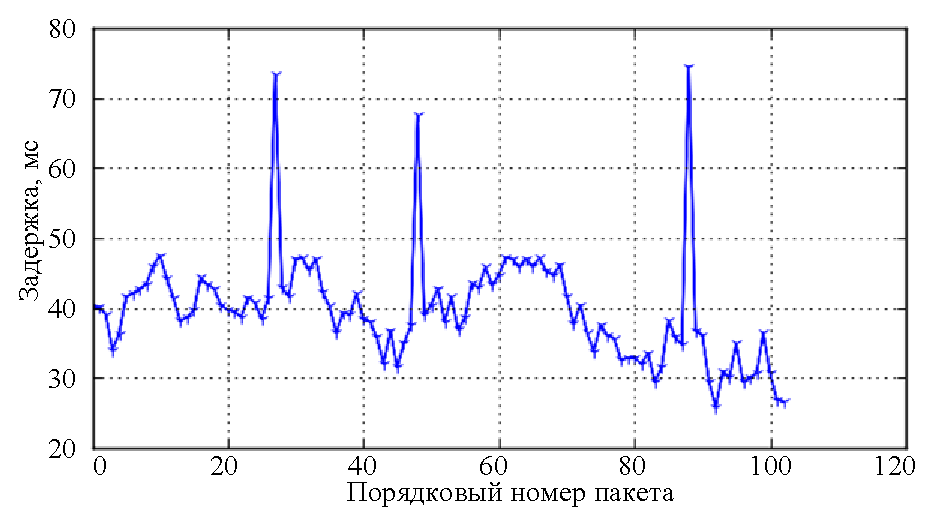
\includegraphics[width=1\linewidth , height=3.5cm]{3chapter/3_1_a.eps} \\{\scriptsize а)} \\
\end{minipage}
\hfill
\begin{minipage}[h]{0.47\linewidth}
\center
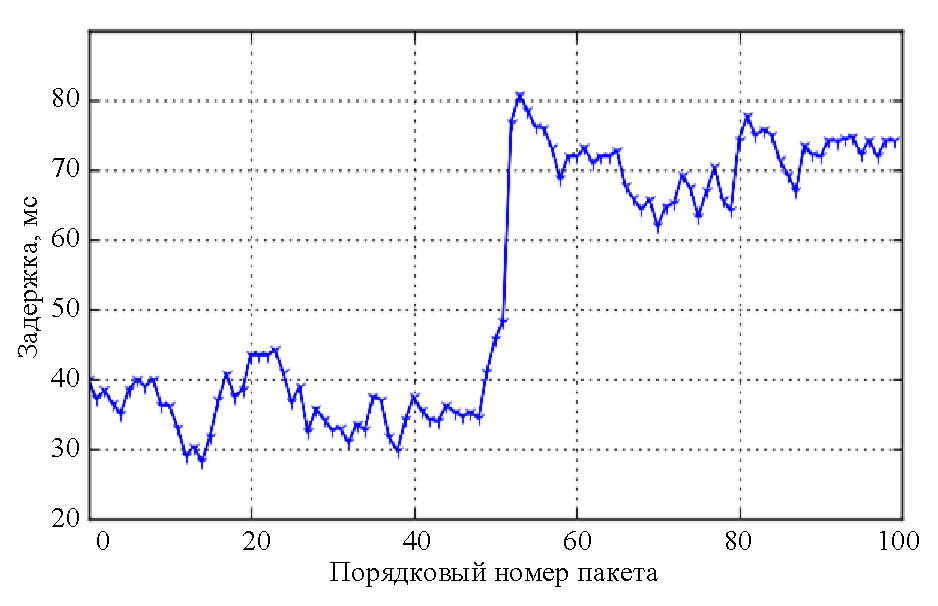
\includegraphics[width=1\linewidth, height=3.5cm]{3chapter/3_1_b.eps} \\{\scriptsize б)} \\
\end{minipage}
\caption*{Моделирование ряда задержек а) с выбросами, б) со скачками}
\label{img3:modelJitter}
\end{figure}
\end{frame}


\section{Третий научный результат}

\begin{frame}
\frametitle{Третий научный результат}

{\Large Разработан новый адаптивный метод компенсации джиттера на базе робастных процедур инвариантных к распределению вероятностей процесса задержки.}

\end{frame}

\section{Фильтр Калмана-Бьюси (ФКБ)}

\begin{frame}
\frametitle{Фильтр Калмана-Бьюси (ФКБ)}

ФКБ синтезирован с учетом того, что наблюдаемый процесс соответствует уравнению (\ref{eq3:modelStat}) и наблюдается на фоне гауссовского белого шума.
 Уравнение оценки в виде условного среднего значения задержки с использованием ФКБ имеет вид:


\begin{equation}\label{eq3:Estim_rel}
\hat{x}(k+1)=\Phi\hat{x}(k)+K(k)\Delta y,
\end{equation}
\noindent где $\Delta y=H\Phi\hat{x}(k)-y(k)$ - невязка, $K(k)$ - коэффициент усиления ФКБ:

\begin{equation}\label{eq3:K}
K(k)=V(k)H^TN_{\nu}^{-1},
\end{equation}
 
\begin{equation}\label{eq3:V}
V(k)=[I-K(k-1)H(k)]V(k,k-1),
\end{equation}


\begin{equation}\label{eq3:Vkk-1}
V(k,k-1)=\Phi^TV(k-1)\Phi+N_\xi,
\end{equation}

\noindent где $V(k)$ - апостериорная дисперсия ошибки оценки, $V(k,k-1)$ - априорная дисперсия ошибки оценки, $I$ - единичная матрица.

\end{frame}

\section{Робастный Фильтр Калмана-Бьюси (РФКБ) для ситуации выброса}

\begin{frame}
\frametitle{Робастный Фильтр Калмана-Бьюси (РФКБ) для ситуации выброса}

\begin{equation}\label{eq3:skachok}
\hat{x}(k+1)=\Phi(k+1,k)\hat{x}(k)+K(k)\Delta y\cdot min\left\{1,\frac{b}{|K(k)\Delta y|}\right\},
\end{equation}
где $b$ аргумент, ограничивающий изменение значения функции.
\begin{figure} [h]
  \center
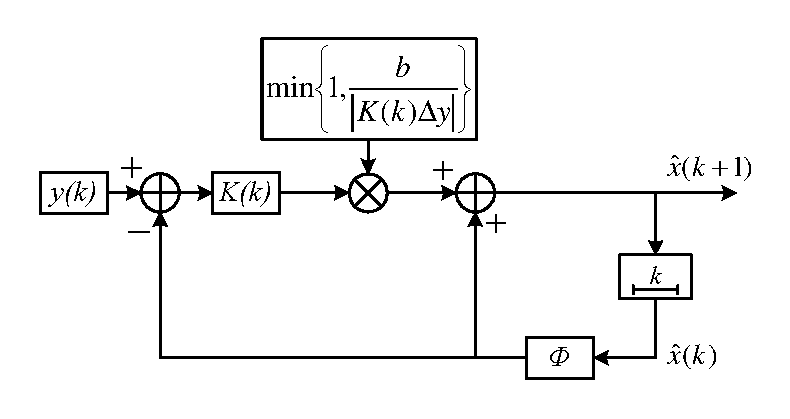
\includegraphics[width=0.8\textwidth]{3chapter/output.eps}
  \caption*{Схема РФКБ для фильтрации случайных процессов содержащих выбросы}
  \label{img3:kalmanV}
\end{figure}

\end{frame}


\section{Робастный Фильтр Калмана-Бьюси (РФКБ) для ситуации скачка}

\begin{frame}
\frametitle{{\large Робастный Фильтр Калмана-Бьюси (РФКБ) для ситуации скачка}}

\begin{equation}\label{eq3:vibros}
\begin{split}
\hat{x}(k+1)=&\Phi(k+1,k)\hat{x}(k)+H(k)[I-H(k)K(k)\Delta y]\times \\
&\times min\left\{1,\frac{b}{|I-H(k)K(k)\Delta y|}\right\},
\end{split}
\end{equation}
\begin{figure} [h]
  \center
\includegraphics[width=0.8\textwidth]{3chapter/output1.eps}
  \caption*{Схема РФКБ для фильтрации случайных процессов содержащих скачки}
  \label{img3:kalmanS}
\end{figure}
\end{frame}


\section{Гибридный Робастный Фильтр Калмана-Бьюси}


\begin{frame}[fragile]
\frametitle{Гибридный Робастный Фильтр Калмана-Бьюси}
\begin{scriptsize}
\begin{equation}\label{eq3:syntes1}
\begin{split}
\hat{x}(k+1)=&\Phi(k+1,k)\hat{x}(k)+(1-\eta)K(k)\Delta y min\left\{1,\frac{b}{|K(k)\Delta y|}\right\}+\\
&+\eta H(k)[I-H(k)K(k)\Delta y] \left\{1,\frac{b}{|I-H(k)K(k)\Delta y|}\right\},
\end{split}
\end{equation}

\begin{equation}\label{eq3:syntes2}
\eta= \;
\begin{cases}
0, \; cond(k) \\    
1, \; cond(k),    
\end{cases}
\end{equation}
где $cond(k)$ - функция, которая определяет, произошел ли скачок задержки:

\begin{lstlisting}[language=Python]
 1  def cond(arr, w, b):  
 2    try:  
 3      arr[-w] 
 4    except IndexError:
 5      return False
 6    if arr[-w]<b:
 7      return False
 8    if w==1 and arr[-w]>=b:
 9      return True
 10   if k==1 and arr[-w]<b:
 11     return False
 12   else:
 13     if cond(arr, w-1, b):
 14       return True  # detected nonstationary delay
 15     else:
 16       return False  # no detected nonstationary delay
\end{lstlisting}
\end{tiny}

\end{frame}






\section{Сравнительный анализ алгоритмов фильтрации}

\begin{frame}
\frametitle{Сравнительный анализ алгоритмов фильтрации}
\begin{scriptsize}

\pgfplotsset{width=10cm, height=4cm, compat=newest}
\begin{figure} [!h]
  \center
\begin{tikzpicture}
%\pgfkeys{/pgfplots/legend pos=north west}

\begin{axis}[
mark options={scale=0.5},
ylabel={Mem [GB]},
legend style={
%area legend,
at={(0.5,-0.2)},
anchor=north,
legend columns=3},
legend cell align=left,
cycle list name=mark list,
%cycle list name=linestyles,
xlabel=Порядковый номер пакета,
ylabel=Задержка (мс),
xmin=380,
xmax=480
]

				\addplot coordinates {
					(1, 20.0)
					(2, 20.5277418762)
					(3, 20.6737546106)
					(4, 20.8417386815)
					(5, 20.8787644691)
					(6, 21.1182037881)
					(7, 20.9261222015)
					(8, 20.7531984604)
					(9, 20.737905212)
					(10, 20.5686348773)
					(11, 20.5976158027)
					(12, 19.8863483394)
					(13, 19.8764026722)
					(14, 20.2062218928)
					(15, 20.2930557777)
					(16, 20.6552595358)
					(17, 20.7520327606)
					(18, 20.8668571972)
					(19, 20.8656243728)
					(20, 20.9541418301)
					(21, 21.177075778)
					(22, 21.7335282945)
					(23, 40.9200404851)
					(24, 20.9200404851)
					(25, 21.1159772503)
					(26, 21.1397573629)
					(27, 21.0959205886)
					(28, 21.1211341993)
					(29, 21.2984304081)
					(30, 21.6289309019)
					(31, 21.4261468128)
					(32, 21.3979378535)
					(33, 21.325869694)
					(34, 21.4983703567)
					(35, 21.2766599276)
					(36, 21.4371025631)
					(37, 21.1993231684)
					(38, 21.165730585)
					(39, 21.0170895854)
					(40, 20.9635259582)
					(41, 21.143490324)
					(42, 20.9445260146)
					(43, 21.5152494372)
					(44, 21.9934078062)
					(45, 22.4621382909)
					(46, 22.2481842679)
					(47, 42.4808875378)
					(48, 22.4808875378)
					(49, 22.557021616)
					(50, 22.5161443098)
					(51, 22.3267695244)
					(52, 22.4886295892)
					(53, 22.4831067366)
					(54, 12.3591429591)
					(55, 12.2333093488)
					(56, 12.1836926318)
					(57, 12.0033149802)
					(58, 11.9392288184)
					(59, 11.6345369611)
					(60, 11.6888292545)
					(61, 11.2515842339)
					(62, 11.7101421062)
					(63, 12.2050200448)
					(64, 11.8913653233)
					(65, 12.4040028855)
					(66, 12.2108745122)
					(67, 11.8821820643)
					(68, 12.1878923569)
					(69, 11.9815339816)
					(70, 31.6516148436)
					(71, 31.7824405141)
					(72, 32.2627891454)
					(73, 32.2084108111)
					(74, 32.0520189432)
					(75, 32.0752132718)
					(76, 31.7489871476)
					(77, 31.8600442526)
					(78, 31.485890523)
					(79, 31.5329563648)
					(80, 31.5745487959)
					(81, 31.4787805569)
					(82, 31.3290660761)
					(83, 31.4437484159)
					(84, 31.1800791206)
					(85, 31.2315166947)
					(86, 31.0357158537)
					(87, 31.4166344923)
					(88, 31.9321873008)
					(89, 32.346733834)
					(90, 52.2704916209)
					(91, 32.2704916209)
					(92, 32.3576897726)
					(93, 32.5595896523)
					(94, 32.636754964)
					(95, 32.7756056459)
					(96, 32.6567073745)
					(97, 32.3885228195)
					(98, 32.232461412)
					(99, 32.1554485132)
					(100, 31.9110121201)
					(101, 31.764267103)
					(102, 31.7061756746)
					(103, 31.5338523276)
					(104, 31.4613247831)
					(105, 31.0153774566)
					(106, 30.5538961657)
					(107, 30.65088987)
					(108, 30.6082039159)
					(109, 30.8150500699)
					(110, 30.4723821761)
					(111, 31.0251337063)
					(112, 30.5794762766)
					(113, 30.73503811)
					(114, 30.7002210406)
					(115, 30.0258986873)
					(116, 29.8814562204)
					(117, 29.7498708146)
					(118, 29.4654006589)
					(119, 29.5909632418)
					(120, 29.6946538059)
					(121, 29.664407229)
					(122, 30.1948499448)
					(123, 29.9004420612)
					(124, 30.0717714021)
					(125, 30.3871116218)
					(126, 30.0456550507)
					(127, 30.3804441742)
					(128, 30.1997275696)
					(129, 30.2535890302)
					(130, 30.1705797262)
					(131, 30.4773188184)
					(132, 30.7789182931)
					(133, 31.1224687037)
					(134, 30.9928320134)
					(135, 30.6696736916)
					(136, 30.7642909423)
					(137, 30.7434321022)
					(138, 30.6471035941)
					(139, 30.7347798383)
					(140, 30.963881555)
					(141, 30.8617823916)
					(142, 31.1280082149)
					(143, 31.0259115411)
					(144, 31.092585319)
					(145, 30.8805490508)
					(146, 30.7725406922)
					(147, 31.1329405297)
					(148, 31.3448424161)
					(149, 31.3728402283)
					(150, 31.4519509753)
					(151, 31.5198068036)
					(152, 31.2114308267)
					(153, 31.3716652118)
					(154, 31.5165944095)
					(155, 32.0534087883)
					(156, 32.0778967282)
					(157, 32.6014773983)
					(158, 32.7681402156)
					(159, 32.3997313036)
					(160, 32.4575134234)
					(161, 32.2362826779)
					(162, 32.3110609039)
					(163, 32.2761300961)
					(164, 32.775174733)
					(165, 33.2615117285)
					(166, 33.3000684415)
					(167, 33.4473618215)
					(168, 33.6793165165)
					(169, 33.6912667109)
					(170, 33.5222008449)
					(171, 33.5313824836)
					(172, 33.3671424199)
					(173, 33.5565273765)
					(174, 33.1133331291)
					(175, 53.0153227815)
					(176, 33.0153227815)
					(177, 33.2298958796)
					(178, 32.8143461129)
					(179, 33.3005624477)
					(180, 33.2961874141)
					(181, 32.9822348255)
					(182, 33.1917425968)
					(183, 32.6211549857)
					(184, 32.6675811647)
					(185, 33.0738740124)
					(186, 32.7065322241)
					(187, 32.7434998791)
					(188, 32.5958317598)
					(189, 33.2708347076)
					(190, 33.5851511847)
					(191, 33.76461767)
					(192, 33.9200738661)
					(193, 33.4325115858)
					(194, 33.2117076527)
					(195, 33.3709517256)
					(196, 33.4511591821)
					(197, 33.3992656319)
					(198, 33.2163426957)
					(199, 33.8470198041)
					(200, 33.5967169985)
					(201, 33.6091914175)
					(202, 32.9791743435)
					(203, 33.2384932221)
					(204, 33.5852619036)
					(205, 33.8144530235)
					(206, 34.2253780984)
					(207, 34.2813307283)
					(208, 34.3818377758)
					(209, 34.0139969255)
					(210, 33.5307619133)
					(211, 33.442328129)
					(212, 33.2891697589)
					(213, 33.2230106159)
					(214, 33.5890457678)
					(215, 33.9433660773)
					(216, 34.4617345678)
					(217, 33.789247433)
					(218, 33.743631486)
					(219, 34.1153698597)
					(220, 34.1241811494)
					(221, 33.7916436664)
					(222, 33.7397898991)
					(223, 33.5575122411)
					(224, 33.6348419452)
					(225, 33.9554158153)
					(226, 33.6548989004)
					(227, 34.1552889685)
					(228, 34.1129402041)
					(229, 34.0941549098)
					(230, 34.3249284335)
					(231, 34.1077476314)
					(232, 34.4015134045)
					(233, 34.9148435961)
					(234, 34.6678874506)
					(235, 34.9418498724)
					(236, 34.9194683764)
					(237, 35.6432729645)
					(238, 35.5786176186)
					(239, 35.4349392849)
					(240, 35.2599381866)
					(241, 35.6267389935)
					(242, 35.9534754068)
					(243, 35.9989518049)
					(244, 35.7146787859)
					(245, 35.6874934996)
					(246, 35.9972017912)
					(247, 36.0986698158)
					(248, 36.1423135058)
					(249, 36.4954997122)
					(250, 36.516444653)
					(251, 36.0909639409)
					(252, 35.8402289916)
					(253, 35.6256411547)
					(254, 35.8828045082)
					(255, 35.9920793407)
					(256, 36.0884159702)
					(257, 36.187283264)
					(258, 36.249544442)
					(259, 36.0887455263)
					(260, 35.7744091058)
					(261, 35.6214659321)
					(262, 35.0918785415)
					(263, 34.4266712872)
					(264, 33.8472520809)
					(265, 34.1226122118)
					(266, 33.4561535633)
					(267, 33.7518834267)
					(268, 33.8844869227)
					(269, 33.7229752571)
					(270, 33.8274152447)
					(271, 33.8330032026)
					(272, 33.4871677405)
					(273, 33.9741006072)
					(274, 34.0261132066)
					(275, 34.3518329587)
					(276, 34.8612523906)
					(277, 35.0876732572)
					(278, 35.1217779853)
					(279, 34.8624664341)
					(280, 34.9471112921)
					(281, 34.8721084368)
					(282, 34.8251447126)
					(283, 34.2514930124)
					(284, 34.0024353537)
					(285, 34.0818221199)
					(286, 34.1554564614)
					(287, 33.9789460333)
					(288, 34.2490532162)
					(289, 33.9145182505)
					(290, 33.9986200823)
					(291, 34.1740251606)
					(292, 34.0928158874)
					(293, 34.2114979105)
					(294, 13.7618736968)
					(295, 13.7298885788)
					(296, 13.6889809952)
					(297, 13.3722758798)
					(298, 13.1993463547)
					(299, 13.6295250851)
					(300, 13.4528188479)
					(301, 13.8605817882)
					(302, 14.0289818694)
					(303, 14.1544021786)
					(304, 13.9991255426)
					(305, 13.7228586449)
					(306, 13.4181353452)
					(307, 13.1142483303)
					(308, 12.9070820476)
					(309, 13.1860203044)
					(310, 13.1459359169)
					(311, 13.0688193201)
					(312, 13.2620448904)
					(313, 13.5729755523)
					(314, 12.954352048)
					(315, 12.7446777807)
					(316, 13.0617895943)
					(317, 13.4878000149)
					(318, 13.4001175586)
					(319, 13.6604306903)
					(320, 13.2449505899)
					(321, 13.313040194)
					(322, 14.0980288939)
					(323, 13.8785386709)
					(324, 13.8592059584)
					(325, 13.8437955362)
					(326, 13.413844819)
					(327, 13.5369078406)
					(328, 13.645971965)
					(329, 13.688665324)
					(330, 13.7138142363)
					(331, 13.4058376893)
					(332, 13.8507277625)
					(333, 14.2773818631)
					(334, 14.3433673452)
					(335, 14.0195188837)
					(336, 13.849523678)
					(337, 13.6669045113)
					(338, 13.2591886964)
					(339, 13.4897530374)
					(340, 13.4848407863)
					(341, 14.1231917618)
					(342, 14.2783161843)
					(343, 13.9685119485)
					(344, 14.2787590132)
					(345, 14.3629757654)
					(346, 14.6191943704)
					(347, 14.3829107813)
					(348, 14.6803850903)
					(349, 14.4258329136)
					(350, 14.4482645933)
					(351, 14.6431960459)
					(352, 14.8340740342)
					(353, 15.0859926619)
					(354, 15.3849670119)
					(355, 15.3255739221)
					(356, 15.3086712613)
					(357, 15.381772394)
					(358, 15.6897187772)
					(359, 15.6193764078)
					(360, 15.491687544)
					(361, 15.2104812341)
					(362, 15.0019856958)
					(363, 15.2118800535)
					(364, 14.9463068196)
					(365, 14.8713641326)
					(366, 15.1639660106)
					(367, 15.2506224493)
					(368, 15.2033805376)
					(369, 15.5762311308)
					(370, 16.0962372532)
					(371, 15.8518723944)
					(372, 16.0501956315)
					(373, 15.697126193)
					(374, 15.8429425038)
					(375, 15.6721785894)
					(376, 15.5866687768)
					(377, 15.7566863815)
					(378, 15.6690086985)
					(379, 16.0094375406)
					(380, 15.9244101932)
					(381, 16.2518019887)
					(382, 16.0954451573)
					(383, 15.9541264833)
					(384, 15.8814249266)
					(385, 15.0922296476)
					(386, 14.4973233888)
					(387, 14.5095060479)
					(388, 14.440600105)
					(389, 14.3646509087)
					(390, 14.0338997853)
					(391, 14.3356362422)
					(392, 14.2811246143)
					(393, 14.1307861622)
					(394, 14.2478459535)
					(395, 14.1869238766)
					(396, 13.9169871062)
					(397, 14.4776028091)
					(398, 14.4122635957)
					(399, 14.7532671288)
					(400, 15.0419452232)
					(401, 34.9569839249)
					(402, 14.9569839249)
					(403, 14.9333931447)
					(404, 15.0013375398)
					(405, 14.9722458258)
					(406, 15.7392892031)
					(407, 15.4945710012)
					(408, 15.4791167982)
					(409, 15.2582427862)
					(410, 15.2375602489)
					(411, 15.6088180972)
					(412, 15.6531652478)
					(413, 15.7094393194)
					(414, 15.4086183654)
					(415, 15.3596776774)
					(416, 15.4705729423)
					(417, 15.748437401)
					(418, 15.5747682384)
					(419, 15.7405894922)
					(420, 15.7630266654)
					(421, 15.6427296398)
					(422, 15.134033167)
					(423, 15.1587223775)
					(424, 15.0446736646)
					(425, 14.742969516)
					(426, 14.111304303)
					(427, 14.0958101615)
					(428, 14.1923888644)
					(429, 14.1863213179)
					(430, 14.0722721041)
					(431, 13.9951693522)
					(432, 13.9239059289)
					(433, 13.6969391038)
					(434, 33.8722887554)
					(435, 33.7776965418)
					(436, 33.9786609691)
					(437, 34.2128435542)
					(438, 33.9381235617)
					(439, 33.9119589944)
					(440, 33.5163257851)
					(441, 33.5254283358)
					(442, 33.581938374)
					(443, 33.7919976503)
					(444, 34.1091696475)
					(445, 34.1013974703)
					(446, 33.977217821)
					(447, 33.7463353106)
					(448, 33.842811131)
					(449, 33.2438542246)
					(450, 33.6476498881)
					(451, 33.3759983419)
					(452, 33.7379735684)
					(453, 34.0685775714)
					(454, 33.8255588977)
					(455, 34.0551943832)
					(456, 34.4800114714)
					(457, 33.9072990865)
					(458, 34.1341356217)
					(459, 33.8369252013)
					(460, 34.2374250708)
					(461, 34.1565924107)
					(462, 33.8369129977)
					(463, 33.9710398678)
					(464, 33.5380574384)
					(465, 33.5688175954)
					(466, 33.8404969457)
					(467, 34.2152255717)
					(468, 34.2205542278)
					(469, 33.7303408327)
					(470, 33.7856428899)
					(471, 34.1976597085)
					(472, 34.2061513643)
					(473, 33.7200650514)
					(474, 33.8069050779)
					(475, 33.9304850265)
					(476, 33.6257368102)
					(477, 33.471074063)
					(478, 33.1080498224)
					(479, 33.275987886)
					(480, 33.2317725263)
					(481, 33.0292396815)
					(482, 32.3476612072)
					(483, 32.1138223573)
					(484, 32.5011608539)
					(485, 32.2153508186)
					(486, 32.2118266721)
					(487, 32.1457371806)
					(488, 31.9327324645)
					(489, 31.9617349311)
					(490, 31.8935243789)
					(491, 31.2513060293)
					(492, 31.0114449066)
					(493, 31.2042625542)
					(494, 30.8271574064)
					(495, 31.3459327681)
					(496, 31.2408010553)
					(497, 31.4710373788)
					(498, 31.3525269464)
					(499, 31.5945950578)
					(500, 31.350712605)
					(501, 31.4296960132)
					(502, 31.3186186362)
					(503, 31.1964385866)
					(504, 31.4029642115)
					(505, 31.1994468521)
				};
				\addplot coordinates {
					(1, 20.0)
					(2, 20.0)
					(3, 20.0022346485)
					(4, 20.0077665215)
					(5, 20.01630003)
					(6, 20.0305379016)
					(7, 20.0448164794)
					(8, 20.0581685622)
					(9, 20.0728676944)
					(10, 20.0848957621)
					(11, 20.0986119717)
					(12, 20.0924369737)
					(13, 20.0856799767)
					(14, 20.0896953241)
					(15, 20.0968522813)
					(16, 20.1174738406)
					(17, 20.1419192008)
					(18, 20.1709037943)
					(19, 20.1996045466)
					(20, 20.2316893182)
					(21, 20.272926544)
					(22, 20.3380863723)
					(23, 21.2747090018)
					(24, 21.2582831456)
					(25, 21.2515893651)
					(26, 21.246256292)
					(27, 21.2389994561)
					(28, 21.2332485565)
					(29, 21.2364592827)
					(30, 21.2559548366)
					(31, 21.2644720262)
					(32, 21.2711953654)
					(33, 21.2739656656)
					(34, 21.2853947772)
					(35, 21.284947872)
					(36, 21.2927640925)
					(37, 21.2879468523)
					(38, 21.2816262071)
					(39, 21.2679069221)
					(40, 21.2520821782)
					(41, 21.2464241342)
					(42, 21.230663636)
					(43, 21.2455458109)
					(44, 21.2847139215)
					(45, 21.3464624141)
					(46, 21.3938081696)
					(47, 22.5021677002)
					(48, 22.501048153)
					(49, 22.5039953317)
					(50, 22.5046354788)
					(51, 22.4952574373)
					(52, 22.4949077829)
					(53, 22.4942849011)
					(54, 21.9590943441)
					(55, 21.4453175865)
					(56, 20.9558900072)
					(57, 20.4826480686)
					(58, 20.0309111955)
					(59, 19.5868421357)
					(60, 19.169041224)
					(61, 18.7501325226)
					(62, 18.3775878162)
					(63, 18.0508973325)
					(64, 17.7248540823)
					(65, 17.4431721851)
					(66, 17.1661498444)
					(67, 16.8863664671)
					(68, 16.6375647103)
					(69, 16.3909929799)
					(70, 17.1992080855)
					(71, 17.9715910244)
					(72, 18.7285439558)
					(73, 19.4425546838)
					(74, 20.1104870537)
					(75, 20.7442887778)
					(76, 21.3272529763)
					(77, 21.8852331923)
					(78, 22.3938451175)
					(79, 22.8780159242)
					(80, 23.3387483734)
					(81, 23.7700050949)
					(82, 24.1704879085)
					(83, 24.5558338003)
					(84, 24.9067980771)
					(85, 25.2418962533)
					(86, 25.5488688954)
					(87, 25.8597618388)
					(88, 26.1815005465)
					(89, 26.5081585477)
					(90, 27.8731544093)
					(91, 28.1061447955)
					(92, 28.3314114214)
					(93, 28.555440811)
					(94, 28.7716893489)
					(95, 28.983837584)
					(96, 29.1784457665)
					(97, 29.3485331195)
					(98, 29.5013396476)
					(99, 29.6419693207)
					(100, 29.7621962113)
					(101, 29.8682775502)
					(102, 29.9656601844)
					(103, 30.048752304)
					(104, 30.1235988441)
					(105, 30.1708506506)
					(106, 30.1911467266)
					(107, 30.2155067248)
					(108, 30.2363142316)
					(109, 30.2669792239)
					(110, 30.2778627435)
					(111, 30.3174578006)
					(112, 30.331341172)
					(113, 30.352731558)
					(114, 30.3711437271)
					(115, 30.352850478)
					(116, 30.3278730458)
					(117, 30.2972468468)
					(118, 30.2531703881)
					(119, 30.2180824706)
					(120, 30.1903479098)
					(121, 30.1624802431)
					(122, 30.164195395)
					(123, 30.1502200708)
					(124, 30.1460633626)
					(125, 30.1588356299)
					(126, 30.1528386038)
					(127, 30.1648985936)
					(128, 30.1667440542)
					(129, 30.1713456535)
					(130, 30.1713050698)
					(131, 30.1875196262)
					(132, 30.2188556931)
					(133, 30.2667348652)
					(134, 30.3052081173)
					(135, 30.3245198255)
					(136, 30.3478217015)
					(137, 30.3687836618)
					(138, 30.3835308258)
					(139, 30.4021422376)
					(140, 30.4319067678)
					(141, 30.4546843192)
					(142, 30.4903613125)
					(143, 30.5187381786)
					(144, 30.5491442596)
					(145, 30.566704199)
					(146, 30.5776107291)
					(147, 30.6070356439)
					(148, 30.6461293526)
					(149, 30.6846351301)
					(150, 30.725292418)
					(151, 30.7673908582)
					(152, 30.7909189283)
					(153, 30.821690571)
					(154, 30.8585110093)
					(155, 30.9218243163)
					(156, 30.9830804077)
					(157, 31.0688334048)
					(158, 31.1588735204)
					(159, 31.2246220819)
					(160, 31.2899485306)
					(161, 31.3400913511)
					(162, 31.3915395126)
					(163, 31.4384107652)
					(164, 31.5092410485)
					(165, 31.6020875284)
					(166, 31.69205739)
					(167, 31.7850646175)
					(168, 31.8854341683)
					(169, 31.9811186975)
					(170, 32.0627750617)
					(171, 32.1405912526)
					(172, 32.2055817588)
					(173, 32.2771634766)
					(174, 32.3214690796)
					(175, 33.4179614758)
					(176, 33.3966271089)
					(177, 33.3877926246)
					(178, 33.3574077698)
					(179, 33.354395742)
					(180, 33.3513114934)
					(181, 33.3317554568)
					(182, 33.3243366822)
					(183, 33.2870776296)
					(184, 33.2542527544)
					(185, 33.2446951379)
					(186, 33.2161798332)
					(187, 33.1911342335)
					(188, 33.1595913104)
					(189, 33.1654856953)
					(190, 33.1877222504)
					(191, 33.2182898504)
					(192, 33.255474845)
					(193, 33.264855381)
					(194, 33.2620392753)
					(195, 33.2678101517)
					(196, 33.2775251532)
					(197, 33.2839757404)
					(198, 33.2803921102)
					(199, 33.3104156606)
					(200, 33.3255857321)
					(201, 33.3406129707)
					(202, 33.3214616462)
					(203, 33.3170654498)
					(204, 33.331276209)
					(205, 33.3568779994)
					(206, 33.4028966757)
					(207, 33.4494417163)
					(208, 33.4988460083)
					(209, 33.5261419906)
					(210, 33.5263867836)
					(211, 33.5219328197)
					(212, 33.5095995477)
					(213, 33.4944142377)
					(214, 33.4994284199)
					(215, 33.5229510693)
					(216, 33.5726938086)
					(217, 33.5841682012)
					(218, 33.5926175835)
					(219, 33.6203163342)
					(220, 33.6470143069)
					(221, 33.6546776931)
					(222, 33.6591874808)
					(223, 33.6538000779)
					(224, 33.6527955551)
					(225, 33.6688303072)
					(226, 33.6680921324)
					(227, 33.6939069291)
					(228, 33.7161099855)
					(229, 33.7361412175)
					(230, 33.7673389207)
					(231, 33.7853759461)
					(232, 33.8180228396)
					(233, 33.8761394011)
					(234, 33.9180912642)
					(235, 33.9723365269)
					(236, 34.0225216151)
					(237, 34.1083993621)
					(238, 34.1863009054)
					(239, 34.2524617332)
					(240, 34.3058442634)
					(241, 34.3758336937)
					(242, 34.4594272171)
					(243, 34.5410010521)
					(244, 34.6031899865)
					(245, 34.6606433046)
					(246, 34.7314627006)
					(247, 34.8039060564)
					(248, 34.8748234222)
					(249, 34.9606971921)
					(250, 35.0431306184)
					(251, 35.0986515131)
					(252, 35.1379450192)
					(253, 35.163786272)
					(254, 35.2018844456)
					(255, 35.2437540126)
					(256, 35.2885095921)
					(257, 35.3361323555)
					(258, 35.3845307555)
					(259, 35.421844547)
					(260, 35.4405256667)
					(261, 35.4501130364)
					(262, 35.4311314873)
					(263, 35.3779087773)
					(264, 35.2968048199)
					(265, 35.234588604)
					(266, 35.140355769)
					(267, 35.0667856458)
					(268, 35.0041399163)
					(269, 34.9362556387)
					(270, 34.8775022001)
					(271, 34.8221579793)
					(272, 34.7514216791)
					(273, 34.7102342493)
					(274, 34.6739851517)
					(275, 34.6569154732)
					(276, 34.6677425468)
					(277, 34.689993155)
					(278, 34.7128718701)
					(279, 34.7207983445)
					(280, 34.7327898484)
					(281, 34.7401718361)
					(282, 34.7446742412)
					(283, 34.7185423532)
					(284, 34.6805984355)
					(285, 34.6488714461)
					(286, 34.6227271722)
					(287, 34.5886155401)
					(288, 34.5706233617)
					(289, 34.5358587269)
					(290, 34.5073923959)
					(291, 34.4897284729)
					(292, 34.4686975117)
					(293, 34.4550694359)
					(294, 33.3586119014)
					(295, 32.318556907)
					(296, 31.331443117)
					(297, 30.3798518559)
					(298, 29.4695190615)
					(299, 28.6302151202)
					(300, 27.8260198327)
					(301, 27.0860418245)
					(302, 26.394195483)
					(303, 25.7456531429)
					(304, 25.1232471668)
					(305, 24.5191818476)
					(306, 23.9309775783)
					(307, 23.3578382512)
					(308, 22.8040905109)
					(309, 22.2944637873)
					(310, 21.8097164124)
					(311, 21.3465679168)
					(312, 20.918198307)
					(313, 20.5290015423)
					(314, 20.1276482853)
					(315, 19.736451404)
					(316, 19.3827852364)
					(317, 19.0704313089)
					(318, 18.7699819094)
					(319, 18.4992452865)
					(320, 18.2208392306)
					(321, 17.9607927255)
					(322, 17.756118853)
					(323, 17.5506599157)
					(324, 17.3550631332)
					(325, 17.1690137738)
					(326, 16.9700409643)
					(327, 16.7881316677)
					(328, 16.6216399995)
					(329, 16.4662322885)
					(330, 16.3203916195)
					(331, 16.1659599572)
					(332, 16.0432841841)
					(333, 15.9497154126)
					(334, 15.8646008433)
					(335, 15.7668366294)
					(336, 15.6652451566)
					(337, 15.5593603196)
					(338, 15.4374825517)
					(339, 15.3342794154)
					(340, 15.2362843573)
					(341, 15.17730561)
					(342, 15.1296714146)
					(343, 15.0681457778)
					(344, 15.0263190306)
					(345, 14.9911708722)
					(346, 14.9714611839)
					(347, 14.9402760286)
					(348, 14.9265053486)
					(349, 14.8999765286)
					(350, 14.8760419483)
					(351, 14.8637042869)
					(352, 14.862134287)
					(353, 14.873995732)
					(354, 14.9010702504)
					(355, 14.9235631633)
					(356, 14.9439686474)
					(357, 14.9671662831)
					(358, 15.0054517242)
					(359, 15.0379813708)
					(360, 15.0620216185)
					(361, 15.0698879561)
					(362, 15.0662900612)
					(363, 15.0740043478)
					(364, 15.0672381181)
					(365, 15.0568594646)
					(366, 15.0625346528)
					(367, 15.0725007443)
					(368, 15.0794355907)
					(369, 15.105758988)
					(370, 15.1582408459)
					(371, 15.1949938707)
					(372, 15.2403079163)
					(373, 15.2645130631)
					(374, 15.2951619453)
					(375, 15.3151386925)
					(376, 15.3295260888)
					(377, 15.3521597664)
					(378, 15.3689484443)
					(379, 15.402885643)
					(380, 15.4305193411)
					(381, 15.4740361356)
					(382, 15.5069623502)
					(383, 15.5306559589)
					(384, 15.5492419367)
					(385, 15.5250265099)
					(386, 15.4705722417)
					(387, 15.4196488231)
					(388, 15.3677725756)
					(389, 15.3146207897)
					(390, 15.2467600198)
					(391, 15.198482869)
					(392, 15.1498753758)
					(393, 15.0958775274)
					(394, 15.0509434041)
					(395, 15.0051621371)
					(396, 14.9475036813)
					(397, 14.9226053351)
					(398, 14.8955641737)
					(399, 14.8880243684)
					(400, 14.8961800773)
					(401, 15.9591294547)
					(402, 15.9060293907)
					(403, 15.8544929169)
					(404, 15.8092873018)
					(405, 15.764935504)
					(406, 15.7635765994)
					(407, 15.7493229665)
					(408, 15.7350057198)
					(409, 15.7097437778)
					(410, 15.6847244819)
					(411, 15.6807024773)
					(412, 15.6792433792)
					(413, 15.6808433528)
					(414, 15.6664191361)
					(415, 15.6501660166)
					(416, 15.6406500297)
					(417, 15.6463612923)
					(418, 15.6425678356)
					(419, 15.6477616483)
					(420, 15.6538691243)
					(421, 15.6532788834)
					(422, 15.6257659325)
					(423, 15.6010189852)
					(424, 15.5715402605)
					(425, 15.5276372962)
					(426, 15.4525909379)
					(427, 15.380700036)
					(428, 15.3177357286)
					(429, 15.2577861746)
					(430, 15.1949700755)
					(431, 15.1313969783)
					(432, 15.0674163986)
					(433, 14.9947997678)
					(434, 15.9950495742)
					(435, 16.9372876653)
					(436, 17.8402483482)
					(437, 18.7077729007)
					(438, 19.5147740495)
					(439, 20.2776287631)
					(440, 20.9790993952)
					(441, 21.6438839491)
					(442, 22.2764382382)
					(443, 22.8866060461)
					(444, 23.4812490665)
					(445, 24.0439722863)
					(446, 24.5702990097)
					(447, 25.0565039567)
					(448, 25.5220585681)
					(449, 25.9312085677)
					(450, 26.3400748603)
					(451, 26.7128829761)
					(452, 27.0851170964)
					(453, 27.4551453873)
					(454, 27.7926905389)
					(455, 28.1245179478)
					(456, 28.4612725432)
					(457, 28.7498377756)
					(458, 29.0351322277)
					(459, 29.2895618553)
					(460, 29.5517312162)
					(461, 29.7957261417)
					(462, 30.0098540044)
					(463, 30.2197429041)
					(464, 30.3955683792)
					(465, 30.5637073683)
					(466, 30.7373325863)
					(467, 30.9216135459)
					(468, 31.0964124707)
					(469, 31.2359748)
					(470, 31.3710724825)
					(471, 31.5208431076)
					(472, 31.6631278715)
					(473, 31.7721175267)
					(474, 31.8799335533)
					(475, 31.988584853)
					(476, 32.0753316089)
					(477, 32.149286949)
					(478, 32.200088323)
					(479, 32.2570963462)
					(480, 32.3087409087)
					(481, 32.3469175306)
					(482, 32.3469569353)
					(483, 32.3346039779)
					(484, 32.3434292239)
					(485, 32.3366428128)
					(486, 32.3300292573)
					(487, 32.3202642873)
					(488, 32.2997303788)
					(489, 32.2818212236)
					(490, 32.2612467794)
					(491, 32.207733675)
					(492, 32.1443466636)
					(493, 32.0945350097)
					(494, 32.0273812583)
					(495, 31.9912737696)
					(496, 31.9515089371)
					(497, 31.9260504885)
					(498, 31.8956615521)
					(499, 31.8797091284)
					(500, 31.8516795176)
					(501, 31.8293201392)
					(502, 31.8022599153)
					(503, 31.7701596361)
					(504, 31.7507032797)
					(505, 31.7214941971)
				};
				\addplot coordinates {
					(1, 20.0)
					(2, 20.0)
					(3, 20.0022346485)
					(4, 20.0077665215)
					(5, 20.01630003)
					(6, 20.0305379016)
					(7, 20.0448164794)
					(8, 20.0581685622)
					(9, 20.0728676944)
					(10, 20.0848957621)
					(11, 20.0986119717)
					(12, 20.0924369737)
					(13, 20.0856799767)
					(14, 20.0896953241)
					(15, 20.0968522813)
					(16, 20.1174738406)
					(17, 20.1419192008)
					(18, 20.1709037943)
					(19, 20.1996045466)
					(20, 20.2316893182)
					(21, 20.272926544)
					(22, 20.3253405605)
					(23, 20.3876345947)
					(24, 20.4122920485)
					(25, 20.4453919721)
					(26, 20.4785050466)
					(27, 20.5083082347)
					(28, 20.5382093329)
					(29, 20.5756562862)
					(30, 20.6279764313)
					(31, 20.6679205499)
					(32, 20.704695161)
					(33, 20.7361695292)
					(34, 20.7749890311)
					(35, 20.8006562557)
					(36, 20.833350645)
					(37, 20.8522179408)
					(38, 20.8684318396)
					(39, 20.8761414639)
					(40, 20.8806845774)
					(41, 20.8943777453)
					(42, 20.8969957202)
					(43, 20.929326778)
					(44, 20.9841630094)
					(45, 21.0441156236)
					(46, 21.1073363821)
					(47, 21.1813321937)
					(48, 21.2497016729)
					(49, 21.3185361763)
					(50, 21.3816398629)
					(51, 21.4314721378)
					(52, 21.4872428434)
					(53, 21.5398064455)
					(54, 21.3479383049)
					(55, 21.0767712176)
					(56, 20.7369604405)
					(57, 20.3395788765)
					(58, 19.8954068468)
					(59, 19.4585043672)
					(60, 19.0474924589)
					(61, 18.6350148421)
					(62, 18.2685619739)
					(63, 17.9476418124)
					(64, 17.6270641992)
					(65, 17.3505592255)
					(66, 17.0784402485)
					(67, 16.8033010493)
					(68, 16.5588979166)
					(69, 16.3164921827)
					(70, 16.8199537064)
					(71, 17.4330026696)
					(72, 18.137748489)
					(73, 18.8830528719)
					(74, 19.5806224543)
					(75, 20.2424924426)
					(76, 20.8520388598)
					(77, 21.4351937961)
					(78, 21.9676473601)
					(79, 22.4743972236)
					(80, 22.9565129338)
					(81, 23.4080203864)
					(82, 23.82768133)
					(83, 24.2311895174)
					(84, 24.5993540246)
					(85, 24.9507412956)
					(86, 25.2731401354)
					(87, 25.5986420683)
					(88, 25.9342158305)
					(89, 26.2739759363)
					(90, 26.9716343476)
					(91, 27.2523912564)
					(92, 27.5228937154)
					(93, 27.7897622944)
					(94, 28.0465803287)
					(95, 28.2971485974)
					(96, 28.5281412158)
					(97, 28.7326852432)
					(98, 28.9181228101)
					(99, 29.0896546041)
					(100, 29.2391462936)
					(101, 29.3729418537)
					(102, 29.4965702816)
					(103, 29.604517566)
					(104, 29.70290232)
					(105, 29.7724451643)
					(106, 29.8138511807)
					(107, 29.8582026001)
					(108, 29.897942272)
					(109, 29.9465362964)
					(110, 29.9743988657)
					(111, 30.0300733238)
					(112, 30.0591841154)
					(113, 30.0949950827)
					(114, 30.1270637445)
					(115, 30.1217033848)
					(116, 30.1089735792)
					(117, 30.0899460528)
					(118, 30.0568536979)
					(119, 30.0321678787)
					(120, 30.0142842487)
					(121, 29.9957455493)
					(122, 30.0062953617)
					(123, 30.0006865826)
					(124, 30.0044531075)
					(125, 30.0247287853)
					(126, 30.0258375918)
					(127, 30.0446269025)
					(128, 30.0528451221)
					(129, 30.0634818114)
					(130, 30.0691565404)
					(131, 30.0907835761)
					(132, 30.1257422104)
					(133, 30.1640725311)
					(134, 30.2079854876)
					(135, 30.2324486701)
					(136, 30.2606290627)
					(137, 30.2862110447)
					(138, 30.3053334322)
					(139, 30.3280882404)
					(140, 30.3617766235)
					(141, 30.388270117)
					(142, 30.4274661582)
					(143, 30.4591756107)
					(144, 30.4927376964)
					(145, 30.5132864152)
					(146, 30.5270233603)
					(147, 30.5591287164)
					(148, 30.6007608397)
					(149, 30.6416705304)
					(150, 30.6846043569)
					(151, 30.7288587101)
					(152, 30.7544284592)
					(153, 30.7871335997)
					(154, 30.8257850868)
					(155, 30.8824692588)
					(156, 30.9458106322)
					(157, 31.0147424312)
					(158, 31.0936840064)
					(159, 31.1628867243)
					(160, 31.2314843061)
					(161, 31.2847249341)
					(162, 31.3391067616)
					(163, 31.3887562359)
					(164, 31.4622175329)
					(165, 31.5575556187)
					(166, 31.649885065)
					(167, 31.7451268513)
					(168, 31.8476125598)
					(169, 31.9453011191)
					(170, 32.0288553271)
					(171, 32.1084688019)
					(172, 32.1751613605)
					(173, 32.2483549452)
					(174, 32.2941870079)
					(175, 32.4168072531)
					(176, 32.4485204243)
					(177, 32.4899226811)
					(178, 32.5071127044)
					(179, 32.549154734)
					(180, 32.5887372915)
					(181, 32.6095873014)
					(182, 32.6404336031)
					(183, 32.639412099)
					(184, 32.6409046758)
					(185, 32.6638461536)
					(186, 32.666107934)
					(187, 32.670208653)
					(188, 32.6662676907)
					(189, 32.6983015084)
					(190, 32.7452924624)
					(191, 32.7993028153)
					(192, 32.8586884161)
					(193, 32.8890932287)
					(194, 32.9061873992)
					(195, 32.9308135784)
					(196, 32.9583848084)
					(197, 32.9817454872)
					(198, 32.9941759441)
					(199, 33.039365053)
					(200, 33.068897115)
					(201, 33.0975253543)
					(202, 33.0912543626)
					(203, 33.0990560168)
					(204, 33.1248183067)
					(205, 33.1613595539)
					(206, 33.2095768459)
					(207, 33.2637371849)
					(208, 33.3229812878)
					(209, 33.359595705)
					(210, 33.3686651828)
					(211, 33.3725683156)
					(212, 33.368149328)
					(213, 33.360458953)
					(214, 33.3725709409)
					(215, 33.4028153089)
					(216, 33.44369419)
					(217, 33.4620038054)
					(218, 33.4769262367)
					(219, 33.5107550532)
					(220, 33.5432582815)
					(221, 33.5564193239)
					(222, 33.5661354669)
					(223, 33.5656785534)
					(224, 33.5693432712)
					(225, 33.5897998577)
					(226, 33.5932492203)
					(227, 33.6218042685)
					(228, 33.6478277838)
					(229, 33.6714770426)
					(230, 33.7053034999)
					(231, 33.7266275576)
					(232, 33.7623873156)
					(233, 33.8022307851)
					(234, 33.8480987982)
					(235, 33.8996870836)
					(236, 33.9537216028)
					(237, 34.0154580354)
					(238, 34.0884848668)
					(239, 34.1598286124)
					(240, 34.2181194364)
					(241, 34.2927570876)
					(242, 34.3807525397)
					(243, 34.466495061)
					(244, 34.5326317983)
					(245, 34.5938237393)
					(246, 34.6681836622)
					(247, 34.7439799452)
					(248, 34.8180725787)
					(249, 34.9069533704)
					(250, 34.9922344872)
					(251, 35.0504521837)
					(252, 35.0922995978)
					(253, 35.1205594362)
					(254, 35.1609480433)
					(255, 35.2049866821)
					(256, 35.2517964022)
					(257, 35.3013644646)
					(258, 35.3516050892)
					(259, 35.3906634926)
					(260, 35.4109967835)
					(261, 35.4221487818)
					(262, 35.4046489573)
					(263, 35.3528294608)
					(264, 35.2816563536)
					(265, 35.2202428002)
					(266, 35.1378911161)
					(267, 35.0644515858)
					(268, 35.0019295297)
					(269, 34.9341623725)
					(270, 34.8755198486)
					(271, 34.8202806653)
					(272, 34.7496438372)
					(273, 34.7085506088)
					(274, 34.6723907213)
					(275, 34.6554055258)
					(276, 34.666312606)
					(277, 34.6886389817)
					(278, 34.7115894495)
					(279, 34.7195838748)
					(280, 34.731639729)
					(281, 34.7390826573)
					(282, 34.7436427741)
					(283, 34.7175655398)
					(284, 34.6796733799)
					(285, 34.6479954058)
					(286, 34.6218975501)
					(287, 34.5878298767)
					(288, 34.5698793278)
					(289, 34.5351541167)
					(290, 34.5067251204)
					(291, 34.4890965539)
					(292, 34.4680990759)
					(293, 34.454502709)
					(294, 34.4125289878)
					(295, 34.1430099054)
					(296, 33.6745010038)
					(297, 33.0344478895)
					(298, 32.246001382)
					(299, 31.3329657955)
					(300, 30.3855615335)
					(301, 29.5099626759)
					(302, 28.6896815429)
					(303, 27.919509706)
					(304, 27.1819189398)
					(305, 26.4687720555)
					(306, 25.7772660585)
					(307, 25.1062985882)
					(308, 24.459906264)
					(309, 23.8625438575)
					(310, 23.294709596)
					(311, 22.7528766872)
					(312, 22.2499918664)
					(313, 21.790228182)
					(314, 21.3220470908)
					(315, 20.8675633405)
					(316, 20.453963646)
					(317, 20.0848518521)
					(318, 19.7306519801)
					(319, 19.4090129277)
					(320, 19.0824015778)
					(321, 18.7767040027)
					(322, 18.5287979451)
					(323, 18.2823975398)
					(324, 18.0480286295)
					(325, 17.8252615369)
					(326, 17.591516534)
					(327, 17.3766774967)
					(328, 17.1790009154)
					(329, 16.9940606672)
					(330, 16.820252283)
					(331, 16.6393348136)
					(332, 16.4915766205)
					(333, 16.3742544555)
					(334, 16.2666450992)
					(335, 16.1475780155)
					(336, 16.0258124349)
					(337, 15.9008224431)
					(338, 15.7608518333)
					(339, 15.6405145294)
					(340, 15.5262931811)
					(341, 15.451947916)
					(342, 15.389761419)
					(343, 15.3144545544)
					(344, 15.2595767968)
					(345, 15.2120691537)
					(346, 15.1806548651)
					(347, 15.1383852939)
					(348, 15.114117521)
					(349, 15.0776478112)
					(350, 15.0442990728)
					(351, 15.0230460754)
					(352, 15.013033131)
					(353, 15.0168989924)
					(354, 15.0364015844)
					(355, 15.0517237798)
					(356, 15.0653384967)
					(357, 15.0821051835)
					(358, 15.1143004283)
					(359, 15.1410625761)
					(360, 15.1596409239)
					(361, 15.1623347679)
					(362, 15.153838451)
					(363, 15.1569138654)
					(364, 15.1457545605)
					(365, 15.131215605)
					(366, 15.1329509304)
					(367, 15.1391859182)
					(368, 15.1425873587)
					(369, 15.1655645725)
					(370, 15.1939562276)
					(371, 15.2288168237)
					(372, 15.2671170508)
					(373, 15.2899016786)
					(374, 15.31920531)
					(375, 15.3379080864)
					(376, 15.3510890148)
					(377, 15.3725801511)
					(378, 15.3882868268)
					(379, 15.4211993546)
					(380, 15.4478626753)
					(381, 15.4883078694)
					(382, 15.5204778765)
					(383, 15.5434553464)
					(384, 15.561363131)
					(385, 15.536505446)
					(386, 15.4935435909)
					(387, 15.4442611696)
					(388, 15.391080803)
					(389, 15.3366939985)
					(390, 15.2737757094)
					(391, 15.224067095)
					(392, 15.1741039863)
					(393, 15.1188223516)
					(394, 15.0726724651)
					(395, 15.0257398537)
					(396, 14.9669910592)
					(397, 14.9410601474)
					(398, 14.9130411323)
					(399, 14.9045752863)
					(400, 14.911854022)
					(401, 14.9698018012)
					(402, 14.9691226284)
					(403, 14.9672294524)
					(404, 14.9690367164)
					(405, 14.9692067555)
					(406, 15.0100106368)
					(407, 15.0356857364)
					(408, 15.0591815432)
					(409, 15.0697290779)
					(410, 15.0786218441)
					(411, 15.1067150243)
					(412, 15.1356694435)
					(413, 15.1660714322)
					(414, 15.1789231162)
					(415, 15.1885006461)
					(416, 15.203446636)
					(417, 15.2323237238)
					(418, 15.250468619)
					(419, 15.2764383499)
					(420, 15.3022209033)
					(421, 15.3202632286)
					(422, 15.3103955718)
					(423, 15.3023589583)
					(424, 15.2887051474)
					(425, 15.2597885918)
					(426, 15.218362692)
					(427, 15.1691945814)
					(428, 15.1174371824)
					(429, 15.0681007233)
					(430, 15.0153353696)
					(431, 14.9612804653)
					(432, 14.9063137438)
					(433, 14.8422333595)
					(434, 14.9190951371)
					(435, 15.2004373157)
					(436, 15.6587709879)
					(437, 16.2710679671)
					(438, 17.0155611402)
					(439, 17.8657470422)
					(440, 18.6950145559)
					(441, 19.4808244972)
					(442, 20.2279914766)
					(443, 20.9466990631)
					(444, 21.6441307323)
					(445, 22.3041962024)
					(446, 22.9227073626)
					(447, 23.4962122269)
					(448, 24.0444410489)
					(449, 24.5318846519)
					(450, 25.0148960535)
					(451, 25.4579205972)
					(452, 25.896650631)
					(453, 26.3296514578)
					(454, 26.7268324585)
					(455, 27.1151358288)
					(456, 27.5053739288)
					(457, 27.8445887685)
					(458, 28.1778490885)
					(459, 28.4777030464)
					(460, 28.7828898667)
					(461, 29.0676229121)
					(462, 29.3203303293)
					(463, 29.5667545925)
					(464, 29.7771795545)
					(465, 29.9780847289)
					(466, 30.1827399706)
					(467, 30.3964067854)
					(468, 30.5990345152)
					(469, 30.7649511019)
					(470, 30.9250066251)
					(471, 31.0984126652)
					(472, 31.2630804891)
					(473, 31.393267207)
					(474, 31.5211571406)
					(475, 31.6488187037)
					(476, 31.7535684379)
					(477, 31.8445728437)
					(478, 31.9115199151)
					(479, 31.9838181336)
					(480, 32.0499427194)
					(481, 32.1018321204)
					(482, 32.1148577139)
					(483, 32.1148028541)
					(484, 32.1352745659)
					(485, 32.1395175167)
					(486, 32.143348917)
					(487, 32.1434754625)
					(488, 32.1323089539)
					(489, 32.1232708539)
					(490, 32.1110974198)
					(491, 32.0655401864)
					(492, 32.0096874933)
					(493, 31.9670109414)
					(494, 31.9066142287)
					(495, 31.8769057477)
					(496, 31.8432008627)
					(497, 31.8234812669)
					(498, 31.7985271023)
					(499, 31.7877214815)
					(500, 31.764565963)
					(501, 31.7468224166)
					(502, 31.7241334483)
					(503, 31.6961728078)
					(504, 31.6806367457)
					(505, 31.6551402351)
				};
				\addplot coordinates {
					(1, 20.0)
					(2, 20.0)
					(3, 20.0022346485)
					(4, 20.0077665215)
					(5, 20.01630003)
					(6, 20.0305379016)
					(7, 20.0448164794)
					(8, 20.0581685622)
					(9, 20.0728676944)
					(10, 20.0848957621)
					(11, 20.0986119717)
					(12, 20.0924369737)
					(13, 20.0856799767)
					(14, 20.0896953241)
					(15, 20.0968522813)
					(16, 20.1174738406)
					(17, 20.1419192008)
					(18, 20.1709037943)
					(19, 20.1996045466)
					(20, 20.2316893182)
					(21, 20.272926544)
					(22, 20.3380863723)
					(23, 37.9200404851)
					(24, 23.9200404851)
					(25, 23.7881430421)
					(26, 23.6618461478)
					(27, 23.5379866776)
					(28, 23.4200632417)
					(29, 23.3155558974)
					(30, 23.2317748367)
					(31, 23.1414129019)
					(32, 23.0535853716)
					(33, 22.9660435352)
					(34, 22.8912937584)
					(35, 22.8086834865)
					(36, 22.7382250672)
					(37, 22.6588887361)
					(38, 22.581667241)
					(39, 22.5005257847)
					(40, 22.4206172767)
					(41, 22.3540741588)
					(42, 22.2804891329)
					(43, 22.2404715671)
					(44, 22.2275319863)
					(45, 22.2398356094)
					(46, 22.2402739636)
					(47, 39.4808875378)
					(48, 25.4808875378)
					(49, 25.3269368083)
					(50, 25.1788321288)
					(51, 25.0284561819)
					(52, 24.8944667549)
					(53, 24.7671905584)
					(54, 15.3591429591)
					(55, 15.1940168887)
					(56, 15.0349372757)
					(57, 14.8746827335)
					(58, 14.7194693776)
					(59, 14.556312877)
					(60, 14.4046244346)
					(61, 14.2377986499)
					(62, 14.1040392256)
					(63, 14.003531379)
					(64, 13.8917278386)
					(65, 13.8129687883)
					(66, 13.728146415)
					(67, 13.6304035517)
					(68, 13.5540171949)
					(69, 13.4707424209)
					(70, 28.6516148436)
					(71, 28.8174351681)
					(72, 29.2627891454)
					(73, 29.4188148311)
					(74, 29.5582975424)
					(75, 29.6916249166)
					(76, 29.8006118677)
					(77, 29.9097113929)
					(78, 29.9932122902)
					(79, 30.0747846784)
					(80, 30.1542404806)
					(81, 30.2244142585)
					(82, 30.2829392617)
					(83, 30.3444402953)
					(84, 30.3887139237)
					(85, 30.4333675579)
					(86, 30.4652816423)
					(87, 30.5156873517)
					(88, 30.5907385592)
					(89, 30.683778008)
					(90, 49.2704916209)
					(91, 35.2704916209)
					(92, 35.1161578322)
					(93, 34.9806984505)
					(94, 34.8565045431)
					(95, 34.7462477356)
					(96, 34.6355327702)
					(97, 34.5164739537)
					(98, 34.3954542919)
					(99, 34.2767661384)
					(100, 34.1514149332)
					(101, 34.0249299825)
					(102, 33.9020687642)
					(103, 33.7765866132)
					(104, 33.6539101913)
					(105, 33.514104822)
					(106, 33.3572550032)
					(107, 33.2138552576)
					(108, 33.0757918607)
					(109, 32.9560038247)
					(110, 32.8244061782)
					(111, 32.7290695471)
					(112, 32.6151707023)
					(113, 32.5155495307)
					(114, 32.4193620578)
					(115, 32.2925413457)
					(116, 32.1647868936)
					(117, 32.0368294281)
					(118, 31.9005789103)
					(119, 31.7782008832)
					(120, 31.6678013828)
					(121, 31.5616488782)
					(122, 31.4892272104)
					(123, 31.4050432984)
					(124, 31.3343980928)
					(125, 31.2842048406)
					(126, 31.2185786041)
					(127, 31.1741689146)
					(128, 31.1225368156)
					(129, 31.0764944342)
					(130, 31.0284933081)
					(131, 30.9992885752)
					(132, 30.9876119545)
					(133, 30.9947575239)
					(134, 30.9946554981)
					(135, 30.9774358915)
					(136, 30.9661421139)
					(137, 30.9543415181)
					(138, 30.9380620946)
					(139, 30.9272909048)
					(140, 30.9292297107)
					(141, 30.9256559218)
					(142, 30.9363778365)
					(143, 30.9411219031)
					(144, 30.9491474008)
					(145, 30.9455126227)
					(146, 30.9363474667)
					(147, 30.946764221)
					(148, 30.9678569428)
					(149, 30.9893155405)
					(150, 31.0138289168)
					(151, 31.0406388528)
					(152, 31.049688501)
					(153, 31.0667488811)
					(154, 31.0905845668)
					(155, 31.1416011362)
					(156, 31.1912120497)
					(157, 31.2659369046)
					(158, 31.3455332194)
					(159, 31.4013913593)
					(160, 31.4573514439)
					(161, 31.4986241901)
					(162, 31.5416722703)
					(163, 31.5805885316)
					(164, 31.6438853298)
					(165, 31.7295974966)
					(166, 31.8128110667)
					(167, 31.899419994)
					(168, 31.9937302673)
					(169, 32.0836765783)
					(170, 32.1598987716)
					(171, 32.2325687287)
					(172, 32.2926856814)
					(173, 32.3596520778)
					(174, 32.3995869083)
					(175, 50.0153227815)
					(176, 36.0153227815)
					(177, 35.8677330931)
					(178, 35.7059451702)
					(179, 35.5784926471)
					(180, 35.4575615547)
					(181, 35.3264029519)
					(182, 35.213295027)
					(183, 35.0759469096)
					(184, 34.9483363269)
					(185, 34.8490153543)
					(186, 34.7354929289)
					(187, 34.6299444281)
					(188, 34.5221641612)
					(189, 34.4558607431)
					(190, 34.4097249956)
					(191, 34.3755430936)
					(192, 34.351409428)
					(193, 34.3027203577)
					(194, 34.2449115439)
					(195, 34.1986035768)
					(196, 34.158999204)
					(197, 34.1187436722)
					(198, 34.070928711)
					(199, 34.0590645886)
					(200, 34.0345664635)
					(201, 34.0120273796)
					(202, 33.9573002361)
					(203, 33.9192132544)
					(204, 33.9015183812)
					(205, 33.8969051031)
					(206, 33.9143096981)
					(207, 33.9337568139)
					(208, 33.957499002)
					(209, 33.9604926225)
					(210, 33.9377227478)
					(211, 33.9114735802)
					(212, 33.8784999534)
					(213, 33.8437679462)
					(214, 33.8302711401)
					(215, 33.8362636314)
					(216, 33.8694050722)
					(217, 33.865157809)
					(218, 33.8587185691)
					(219, 33.8723175919)
					(220, 33.8856629301)
					(221, 33.8806811897)
					(222, 33.8732158702)
					(223, 33.8564878777)
					(224, 33.8447436621)
					(225, 33.8506077789)
					(226, 33.8402378738)
					(227, 33.8569312909)
					(228, 33.8704962765)
					(229, 33.8823471378)
					(230, 33.9057979186)
					(231, 33.9164985028)
					(232, 33.9421976867)
					(233, 33.9937346726)
					(234, 34.0294555879)
					(235, 34.0778000582)
					(236, 34.1223970156)
					(237, 34.2029827267)
					(238, 34.27587264)
					(239, 34.3372873857)
					(240, 34.3861753118)
					(241, 34.4519082905)
					(242, 34.5314708964)
					(243, 34.6092273976)
					(244, 34.667801265)
					(245, 34.7218310653)
					(246, 34.7894083434)
					(247, 34.8587813694)
					(248, 34.926791091)
					(249, 35.0099112822)
					(250, 35.089737032)
					(251, 35.1427884216)
					(252, 35.1797432727)
					(253, 35.2033697873)
					(254, 35.2393705737)
					(255, 35.2792538865)
					(256, 35.3221284562)
					(257, 35.3679698777)
					(258, 35.4146813226)
					(259, 35.4503975447)
					(260, 35.4675657444)
					(261, 35.4757203583)
					(262, 35.4553819699)
					(263, 35.4008743147)
					(264, 35.3185534965)
					(265, 35.255184897)
					(266, 35.159860739)
					(267, 35.085257118)
					(268, 35.021632652)
					(269, 34.9528214977)
					(270, 34.8931902942)
					(271, 34.8370148181)
					(272, 34.7654913078)
					(273, 34.7235583793)
					(274, 34.6866032843)
					(275, 34.6688650166)
					(276, 34.6790589271)
					(277, 34.7007099213)
					(278, 34.7230207938)
					(279, 34.7304095135)
					(280, 34.7418917563)
					(281, 34.7487914668)
					(282, 34.7528371489)
					(283, 34.726272738)
					(284, 34.6879192152)
					(285, 34.6558043241)
					(286, 34.6292927021)
					(287, 34.5948331863)
					(288, 34.5765115574)
					(289, 34.5414349284)
					(290, 34.5126731347)
					(291, 34.4947294044)
					(292, 34.4734334621)
					(293, 34.4595544454)
					(294, 16.7618736968)
					(295, 16.6012197809)
					(296, 16.4469107897)
					(297, 16.2839970158)
					(298, 16.1205525435)
					(299, 15.9885620158)
					(300, 15.8542021645)
					(301, 15.7485674375)
					(302, 15.657452823)
					(303, 15.5778116103)
					(304, 15.4941627503)
					(305, 15.4003077577)
					(306, 15.2952796169)
					(307, 15.1797146642)
					(308, 15.0592960886)
					(309, 14.9600379859)
					(310, 14.8639152841)
					(311, 14.7687996471)
					(312, 14.6889621669)
					(313, 14.629830076)
					(314, 14.5410525604)
					(315, 14.4458691635)
					(316, 14.3725317974)
					(317, 14.3256530629)
					(318, 14.2766122869)
					(319, 14.2439630546)
					(320, 14.1910290005)
					(321, 14.1445075519)
					(322, 14.142044816)
					(323, 14.1280825793)
					(324, 14.1138357804)
					(325, 14.0995273254)
					(326, 14.0631954915)
					(327, 14.035309414)
					(328, 14.014679832)
					(329, 13.9974055033)
					(330, 13.9823790287)
					(331, 13.9518301901)
					(332, 13.9464731385)
					(333, 13.9640067939)
					(334, 13.9841077363)
					(335, 13.9859840448)
					(336, 13.9787535039)
					(337, 13.9622297547)
					(338, 13.924978154)
					(339, 13.9019171505)
					(340, 13.8798177838)
					(341, 13.8927132899)
					(342, 13.9131449914)
					(343, 13.916078686)
					(344, 13.9352958037)
					(345, 13.9579570167)
					(346, 13.9929935904)
					(347, 14.0136538909)
					(348, 14.0489815637)
					(349, 14.0689495525)
					(350, 14.0890480834)
					(351, 14.118410378)
					(352, 14.1563308045)
					(353, 14.205590221)
					(354, 14.2680811279)
					(355, 14.324113843)
					(356, 14.3762819766)
					(357, 14.429559274)
					(358, 14.4963305644)
					(359, 14.5558366983)
					(360, 14.6054240469)
					(361, 14.637483837)
					(362, 14.6567974711)
					(363, 14.6862092877)
					(364, 14.6999909144)
					(365, 14.7090713609)
					(366, 14.7331745817)
					(367, 14.7605922711)
					(368, 14.7840540185)
					(369, 14.826028616)
					(370, 14.8933323737)
					(371, 14.9441219395)
					(372, 15.0027287806)
					(373, 15.0395223858)
					(374, 15.0820927095)
					(375, 15.1133592242)
					(376, 15.1384381841)
					(377, 15.1711969181)
					(378, 15.1975741623)
					(379, 15.2405918638)
					(380, 15.2768249217)
					(381, 15.3284854271)
					(382, 15.3691238469)
					(383, 15.400121019)
					(384, 15.4256235707)
					(385, 15.4079582336)
					(386, 15.3597069896)
					(387, 15.3146579194)
					(388, 15.2683447598)
					(389, 15.2204612939)
					(390, 15.1575896949)
					(391, 15.1140373568)
					(392, 15.0699043257)
					(393, 15.0201438537)
					(394, 14.9792225836)
					(395, 14.9372415432)
					(396, 14.8831819538)
					(397, 14.8616917831)
					(398, 14.8378782104)
					(399, 14.8333949754)
					(400, 14.8444452981)
					(401, 31.9569839249)
					(402, 17.9569839249)
					(403, 17.7967747946)
					(404, 17.6486546937)
					(405, 17.5068414762)
					(406, 17.4131852796)
					(407, 17.3115248543)
					(408, 17.2144321845)
					(409, 17.1107807896)
					(410, 17.011525614)
					(411, 16.9372012204)
					(412, 16.8691648023)
					(413, 16.8077151471)
					(414, 16.7335820733)
					(415, 16.6607838527)
					(416, 16.5977188851)
					(417, 16.5527185336)
					(418, 16.5009004875)
					(419, 16.4606143601)
					(420, 16.4236517134)
					(421, 16.3822734796)
					(422, 16.316133744)
					(423, 16.2548067054)
					(424, 16.1906861362)
					(425, 16.1139768731)
					(426, 16.0078625031)
					(427, 15.906549771)
					(428, 15.8157225897)
					(429, 15.7293865146)
					(430, 15.6415820206)
					(431, 15.5543445732)
					(432, 15.4679535315)
					(433, 15.3741138879)
					(434, 30.8722887554)
					(435, 31.0262357967)
					(436, 31.182674119)
					(437, 31.3432318284)
					(438, 31.480725748)
					(439, 31.6095479969)
					(440, 31.7105812495)
					(441, 31.806743427)
					(442, 31.9008045812)
					(443, 32.0010120559)
					(444, 32.1127156954)
					(445, 32.2180887437)
					(446, 32.3112986256)
					(447, 32.3873360249)
					(448, 32.464456382)
					(449, 32.5057538523)
					(450, 32.5662587897)
					(451, 32.6091639574)
					(452, 32.6689754925)
					(453, 32.7431353402)
					(454, 32.8004890462)
					(455, 32.8669713401)
					(456, 32.9524404976)
					(457, 33.0030349977)
					(458, 33.0629679252)
					(459, 33.1039771196)
					(460, 33.1640344236)
					(461, 33.2166264783)
					(462, 33.2494932156)
					(463, 33.2877253608)
					(464, 33.3009895514)
					(465, 33.3151807899)
					(466, 33.3430153914)
					(467, 33.3892306515)
					(468, 33.4332794785)
					(469, 33.4490196843)
					(470, 33.4668561294)
					(471, 33.5055787656)
					(472, 33.5426995716)
					(473, 33.5520975264)
					(474, 33.5655988561)
					(475, 33.5849328534)
					(476, 33.5870949074)
					(477, 33.5809473828)
					(478, 33.555890253)
					(479, 33.5410592398)
					(480, 33.5246712564)
					(481, 33.4984201307)
					(482, 33.437445581)
					(483, 33.3673115778)
					(484, 33.3214173863)
					(485, 33.2628109228)
					(486, 33.2071230718)
					(487, 33.1508840756)
					(488, 33.0863386313)
					(489, 33.0267499522)
					(490, 32.9667044313)
					(491, 32.8758116795)
					(492, 32.7770256331)
					(493, 32.6936906108)
					(494, 32.594789773)
					(495, 32.5286173611)
					(496, 32.4603806369)
					(497, 32.407958919)
					(498, 32.3520353993)
					(499, 32.3119013775)
					(500, 32.2609714639)
					(501, 32.2169251869)
					(502, 32.1693271746)
					(503, 32.1177773301)
					(504, 32.0799019705)
					(505, 32.0332498409)
				};
				\addplot coordinates {
					(1, 20.0)
					(2, 20.0)
					(3, 20.0022346485)
					(4, 20.0077665215)
					(5, 20.01630003)
					(6, 20.0291437412)
					(7, 20.0434445466)
					(8, 20.0568224885)
					(9, 20.0715507292)
					(10, 20.0836107485)
					(11, 20.0973613346)
					(12, 20.091222719)
					(13, 20.0845037008)
					(14, 20.088558231)
					(15, 20.0957552063)
					(16, 20.1111189929)
					(17, 20.1273598277)
					(18, 20.1447751271)
					(19, 20.1637110008)
					(20, 20.1838841366)
					(21, 20.2054877846)
					(22, 20.2293569347)
					(23, 20.2578826437)
					(24, 20.2885493337)
					(25, 20.3274698635)
					(26, 20.3662064377)
					(27, 20.4014303778)
					(28, 20.4365462767)
					(29, 20.4790009467)
					(30, 20.5361223291)
					(31, 20.5806632496)
					(32, 20.621833446)
					(33, 20.6575063445)
					(34, 20.7003322257)
					(35, 20.7298191516)
					(36, 20.7661524589)
					(37, 20.7884840805)
					(38, 20.8079940963)
					(39, 20.818838117)
					(40, 20.8263604272)
					(41, 20.8428840876)
					(42, 20.8481902731)
					(43, 20.8752058788)
					(44, 20.9021798296)
					(45, 20.9313730462)
					(46, 20.964716903)
					(47, 21.0004768338)
					(48, 21.0783610958)
					(49, 21.156217219)
					(50, 21.2278737238)
					(51, 21.2858133694)
					(52, 21.3492683535)
					(53, 21.4091145132)
					(54, 21.3189661061)
					(55, 21.194836392)
					(56, 21.0407946084)
					(57, 20.860952329)
					(58, 20.6584029364)
					(59, 20.4365636003)
					(60, 20.1973348513)
					(61, 19.9442710242)
					(62, 19.6781114224)
					(63, 12.479080341)
					(64, 12.4479707511)
					(65, 12.4456431251)
					(66, 12.4332133753)
					(67, 12.4040365507)
					(68, 12.3925909082)
					(69, 12.3708223625)
					(70, 12.5027469629)
					(71, 12.7145849506)
					(72, 12.9963416576)
					(73, 13.3406197972)
					(74, 13.7379235152)
					(75, 14.1791212641)
					(76, 14.6568557432)
					(77, 15.1627227418)
					(78, 15.6913723082)
					(79, 30.9887721553)
					(80, 31.0198059374)
					(81, 31.0441222897)
					(82, 31.0592187533)
					(83, 31.0795915869)
					(84, 31.0849155948)
					(85, 31.0926828591)
					(86, 31.0896645891)
					(87, 31.1069884978)
					(88, 31.1507104666)
					(89, 31.2140804291)
					(90, 31.3749962029)
					(91, 31.4224435133)
					(92, 31.4719972097)
					(93, 31.5296231322)
					(94, 31.5882845415)
					(95, 31.6511949667)
					(96, 31.7044723637)
					(97, 31.7407170798)
					(98, 31.766772424)
					(99, 31.7873666777)
					(100, 31.7939181218)
					(101, 31.7923470387)
					(102, 31.7877811738)
					(103, 31.7743265177)
					(104, 31.7577418134)
					(105, 31.7184068748)
					(106, 31.6684855327)
					(107, 31.6189818049)
					(108, 31.5705780647)
					(109, 31.5305455342)
					(110, 31.4852866274)
					(111, 31.4609048676)
					(112, 31.4193232877)
					(113, 31.3830655837)
					(114, 31.3468842031)
					(115, 31.309245604)
					(116, 31.2697069022)
					(117, 31.2279715912)
					(118, 31.1838540136)
					(119, 31.1364382786)
					(120, 31.0869850566)
					(121, 31.036504565)
					(122, 30.9919083703)
					(123, 30.9428271929)
					(124, 30.8966731296)
					(125, 30.8696733254)
					(126, 30.8262558249)
					(127, 30.8026338899)
					(128, 30.7706880792)
					(129, 30.7432888821)
					(130, 30.7129431065)
					(131, 30.7004582319)
					(132, 30.7046155455)
					(133, 30.726756067)
					(134, 30.7408544655)
					(135, 30.7370828546)
					(136, 30.7385245125)
					(137, 30.7387845478)
					(138, 30.7339267065)
					(139, 30.7339719109)
					(140, 30.7461539896)
					(141, 30.7522807195)
					(142, 30.7638242418)
					(143, 30.7758034613)
					(144, 30.7875957149)
					(145, 30.7925209754)
					(146, 30.7914622926)
					(147, 30.801081434)
					(148, 30.811205574)
					(149, 30.8227830013)
					(150, 30.8357214235)
					(151, 30.8501883828)
					(152, 30.8662673991)
					(153, 30.8821427506)
					(154, 30.8985606722)
					(155, 30.9160986119)
					(156, 30.9372185497)
					(157, 30.9615074858)
					(158, 30.9910815992)
					(159, 31.0259921121)
					(160, 31.0635820594)
					(161, 31.1036308698)
					(162, 31.144537082)
					(163, 31.1863671679)
					(164, 32.7329154428)
					(165, 32.7609238464)
					(166, 32.7894911667)
					(167, 32.8243493511)
					(168, 32.8621144994)
					(169, 32.89943384)
					(170, 32.9324320092)
					(171, 32.9641682266)
					(172, 32.9855203703)
					(173, 33.0157759645)
					(174, 33.0209451655)
					(175, 33.0481804089)
					(176, 33.0464394021)
					(177, 33.0561600968)
					(178, 33.0433472491)
					(179, 33.0569761514)
					(180, 33.0696510903)
					(181, 33.0650192188)
					(182, 33.0717338319)
					(183, 33.0478592899)
					(184, 33.0277097286)
					(185, 33.0301558069)
					(186, 33.0130081648)
					(187, 32.9987278963)
					(188, 32.9773798885)
					(189, 32.9929289971)
					(190, 33.0210768955)
					(191, 33.0486674176)
					(192, 33.0765268283)
					(193, 33.0953891719)
					(194, 33.1015524672)
					(195, 33.1158269587)
					(196, 33.1335949993)
					(197, 33.1476719244)
					(198, 33.15131054)
					(199, 33.1691518286)
					(200, 33.1882415024)
					(201, 33.2070827928)
					(202, 33.1950067491)
					(203, 33.1973109399)
					(204, 33.2127591132)
					(205, 33.2282160197)
					(206, 33.2447492824)
					(207, 33.2642016977)
					(208, 33.2864054683)
					(209, 33.311421948)
					(210, 33.3230439787)
					(211, 33.3293644141)
					(212, 33.3272346448)
					(213, 33.3217121908)
					(214, 33.3358772293)
					(215, 33.3519593879)
					(216, 33.3690687208)
					(217, 33.3895882631)
					(218, 33.4083477318)
					(219, 33.4276665044)
					(220, 33.4481055409)
					(221, 33.4663083826)
					(222, 33.4807991782)
					(223, 33.4848639257)
					(224, 33.4928107181)
					(225, 33.5086186528)
					(226, 33.5163695136)
					(227, 33.5312277621)
					(228, 33.5474233268)
					(229, 33.5645030082)
					(230, 33.5821813873)
					(231, 33.6014520961)
					(232, 33.6209417976)
					(233, 33.6419955929)
					(234, 33.6668871728)
					(235, 33.6937967645)
					(236, 33.7237174707)
					(237, 33.7560264468)
					(238, 33.7938945782)
					(239, 33.8361421491)
					(240, 33.8813139972)
					(241, 33.9279583445)
					(242, 35.903934478)
					(243, 35.9089691022)
					(244, 35.8986743616)
					(245, 35.8874846522)
					(246, 35.8932981663)
					(247, 35.9041800665)
					(248, 35.9167978955)
					(249, 35.9448273039)
					(250, 35.9722465454)
					(251, 35.9785369504)
					(252, 35.9712085123)
					(253, 35.952898149)
					(254, 35.9491841407)
					(255, 35.9514570021)
					(256, 35.958713962)
					(257, 35.9708250219)
					(258, 35.9851438354)
					(259, 35.990633314)
					(260, 35.9791763759)
					(261, 35.9669825383)
					(262, 35.9545243782)
					(263, 35.9392479681)
					(264, 35.9182418438)
					(265, 35.8894015056)
					(266, 35.8551880616)
					(267, 35.8130850583)
					(268, 35.7657284072)
					(269, 35.7146483469)
					(270, 35.6597395284)
					(271, 35.6022581466)
					(272, 33.5465976311)
					(273, 33.5692494663)
					(274, 33.5934570221)
					(275, 33.6336406177)
					(276, 33.6829892486)
					(277, 33.7323073594)
					(278, 33.7824841264)
					(279, 33.8333361507)
					(280, 33.8832315835)
					(281, 33.9324589629)
					(282, 33.9797591493)
					(283, 33.9941573431)
					(284, 33.9945959649)
					(285, 33.9992177631)
					(286, 34.0074962861)
					(287, 34.0059835116)
					(288, 34.0188628953)
					(289, 34.0133340503)
					(290, 34.0125544104)
					(291, 34.021110161)
					(292, 34.0249095878)
					(293, 34.0347962276)
					(294, 34.0203632332)
					(295, 33.9063697504)
					(296, 33.7051730797)
					(297, 33.428039049)
					(298, 33.0838822862)
					(299, 32.6816016552)
					(300, 32.2323343172)
					(301, 31.7430814823)
					(302, 31.2231264892)
					(303, 14.6979332956)
					(304, 14.6609060024)
					(305, 14.6112022686)
					(306, 14.5479859711)
					(307, 14.4720174036)
					(308, 14.389097144)
					(309, 14.3253504573)
					(310, 14.2628575502)
					(311, 14.1995897867)
					(312, 14.1499126765)
					(313, 14.1193428668)
					(314, 14.0576142204)
					(315, 13.9880464712)
					(316, 13.9389674723)
					(317, 13.9150617419)
					(318, 13.8877767137)
					(319, 13.8757304709)
					(320, 13.8423077284)
					(321, 13.8142637576)
					(322, 13.829299445)
					(323, 13.8319084533)
					(324, 13.8333548493)
					(325, 13.8339080635)
					(326, 13.8116504328)
					(327, 13.7970928174)
					(328, 13.7890854704)
					(329, 13.7837645704)
					(330, 13.7800581554)
					(331, 13.7602295676)
					(332, 13.7650247393)
					(333, 13.7883663776)
					(334, 13.8113520967)
					(335, 13.8223821012)
					(336, 13.8238202351)
					(337, 13.815505839)
					(338, 13.7984727845)
					(339, 13.7821148426)
					(340, 13.7663633665)
					(341, 13.782740853)
					(342, 13.7988552957)
					(343, 13.8078447876)
					(344, 13.8231988331)
					(345, 13.8389881941)
					(346, 13.8555027696)
					(347, 13.8738540541)
					(348, 13.892548468)
					(349, 13.9129387354)
					(350, 13.9334466416)
					(351, 13.9540676888)
					(352, 13.9756598521)
					(353, 15.0626994872)
					(354, 15.0797752768)
					(355, 15.0927992572)
					(356, 15.1042375333)
					(357, 15.1189431009)
					(358, 15.1384971944)
					(359, 15.1584609047)
					(360, 15.176117378)
					(361, 15.1779381944)
					(362, 15.1686151084)
					(363, 15.1709075612)
					(364, 15.159006781)
					(365, 15.1457363069)
					(366, 15.1467022329)
					(367, 15.152208589)
					(368, 15.1549200053)
					(369, 15.1644427003)
					(370, 15.1748816142)
					(371, 15.1886746365)
					(372, 15.204128485)
					(373, 15.2219582073)
					(374, 15.240024203)
					(375, 15.2589368706)
					(376, 15.276302198)
					(377, 15.2943115441)
					(378, 15.3124716429)
					(379, 15.3302352151)
					(380, 15.3492631703)
					(381, 15.3688835059)
					(382, 15.3905639937)
					(383, 15.4131672288)
					(384, 15.435762872)
					(385, 15.41756029)
					(386, 15.3964942071)
					(387, 15.3734602002)
					(388, 15.3488705033)
					(389, 15.322690218)
					(390, 15.2948613704)
					(391, 15.2640671766)
					(392, 15.2323261314)
					(393, 15.199638004)
					(394, 15.1655281927)
					(395, 14.2215289217)
					(396, 14.2053923533)
					(397, 14.2198158)
					(398, 14.230012912)
					(399, 14.2568946802)
					(400, 14.2830324985)
					(401, 14.3098283421)
					(402, 14.3441187738)
					(403, 14.3753422896)
					(404, 14.4085115119)
					(405, 14.4383817525)
					(406, 14.5073121291)
					(407, 14.5596234029)
					(408, 14.6083440295)
					(409, 14.642779812)
					(410, 14.6742950743)
					(411, 14.7238120664)
					(412, 14.7730551273)
					(413, 14.822670736)
					(414, 14.8537179798)
					(415, 14.8805269526)
					(416, 14.9117913537)
					(417, 14.954250327)
					(418, 14.9871293249)
					(419, 15.0263998923)
					(420, 15.0645289396)
					(421, 15.0951657017)
					(422, 15.097225148)
					(423, 15.1004836636)
					(424, 15.0975264938)
					(425, 15.078739803)
					(426, 15.055661336)
					(427, 15.0306305)
					(428, 15.0039292625)
					(429, 14.9763744716)
					(430, 14.9481759898)
					(431, 14.9189818064)
					(432, 14.8886718627)
					(433, 14.8571752826)
					(434, 14.890693454)
					(435, 15.0150974213)
					(436, 15.2183859082)
					(437, 15.4910811519)
					(438, 15.8246617784)
					(439, 16.2087800386)
					(440, 16.6353200024)
					(441, 17.0950801995)
					(442, 17.5818209135)
					(443, 33.2836652346)
					(444, 33.3274057252)
					(445, 33.368416746)
					(446, 33.4006749111)
					(447, 33.4189902044)
					(448, 33.4414469411)
					(449, 33.4309772183)
					(450, 33.4424579188)
					(451, 33.4389364664)
					(452, 33.4547813599)
					(453, 33.4873041993)
					(454, 33.5052270913)
					(455, 33.5343678672)
					(456, 33.5844740987)
					(457, 33.6015794262)
					(458, 33.6297976512)
					(459, 33.6407725903)
					(460, 33.6723870454)
					(461, 33.6980433349)
					(462, 33.7054015356)
					(463, 33.7194767493)
					(464, 33.7098639967)
					(465, 33.7023904585)
					(466, 33.7097082213)
					(467, 33.7364937558)
					(468, 33.7621423679)
					(469, 33.7604573197)
					(470, 33.7617918119)
					(471, 33.7848868739)
					(472, 33.8072081543)
					(473, 33.8025907567)
					(474, 33.802819357)
					(475, 33.8095838987)
					(476, 33.799842507)
					(477, 33.7844377008)
					(478, 33.7693146532)
					(479, 33.7527000471)
					(480, 33.735695633)
					(481, 33.718212133)
					(482, 33.6993817907)
					(483, 33.6760524866)
					(484, 33.6477115484)
					(485, 33.6170387693)
					(486, 33.5830382839)
					(487, 33.5462617987)
					(488, 33.5068958686)
					(489, 33.4643830331)
					(490, 33.4194584974)
					(491, 31.2984692913)
					(492, 31.2832609082)
					(493, 31.2790750714)
					(494, 31.2551295902)
					(495, 31.2599409219)
					(496, 31.2589267697)
					(497, 31.270165743)
					(498, 31.2745297651)
					(499, 31.2914888663)
					(500, 31.2946269178)
					(501, 31.3017837403)
					(502, 31.3026757605)
					(503, 31.2970466372)
					(504, 31.302658826)
					(505, 31.2971899972)
				};


\legend{Задержка, ФКБ, РФКБ(выбросы), РФКБ(скачки), ГРФКБ}
\end{axis}
\end{tikzpicture}
\caption*{СКО оценки фильтров в разных ситуациях зашумленности}


\begin{tabular}{|p{1.5cm}|p{1.5cm}|p{1.5cm}|p{1.5cm}|p{1.5cm}|}
    \hline
    Тип фильтра        & Условия без выбросов и скачков & Условия с выбросами & Условия со скачками  & Условия с выбросами и скачками \\ \hline
    ФКБ                 & \textbf{0,1327}                 & 0,1722                   & 0,6024                 & 0,2371                           \\ \hline
    РФКБ (для выбросов) & 0,1685                          &  \textbf{0,163}       & 0,6515                 & 0,3052                           \\ \hline
    РФКБ (для скачков)   & 0,135                           & 0,19               & \textbf{0,5024}                & 0,2630                             \\ \hline
    ГРФКБ               & 0,139                          & 0,168               &   0,5523            & \textbf{0,1869}                           \\ \hline
    \end{tabular}
\end{figure}
\end{scriptsize}
\end{frame}


\section{Управления буфером компенсации джиттера (управление состоянием)}

\begin{frame}
\frametitle{Управления буфером компенсации джиттера (управление состоянием)}

\begin{scriptsize}
\begin{figure}[!h]
\centering
\includegraphics[height=3cm]{timing_buffer.png}
\label{fig:man_5}
\end{figure}

Размер буфера $\Delta t^i$ рассчитывается только для первого пакета каждого речевого потока на основе оценки отклонения $\hat V (k)$ от условного среднего значения сетевой задержки:
\begin{equation}\label{eq41:syntes3}
\hat{V}(k)=\alpha\cdot\hat{V}(k-1)+(1-\alpha)\cdot V(k),
\end{equation}

\begin{equation}\label{eq41:syntes4}
V^i(k)= \;
\begin{cases}
| \hat{x}(k)-x(k) |, \; K(k)\Delta y \leq b; \\    
V(k-1), \;  K(k)\Delta y > b,    
\end{cases}
\end{equation}

\begin{equation}\label{eq41:syntes5}
\Delta t^i= \;
\begin{cases}
\gamma\cdot\hat{V}^{i-1}, \; \hat{V}^{i-1} \geq \Delta t_{min}; \\    
\gamma\cdot\Delta t_{min}, \;  \hat{V}^{i-1} < \Delta t_{min},    
\end{cases}
\end{equation}
\noindent где $\gamma$ - константа для управления процентом отбрасываемых пакетов и задержкой.
\end{scriptsize}

\end{frame}

\section{Управления буфером компенсации джиттера (управление состоянием)}

\begin{frame}
\frametitle{Управления буфером компенсации джиттера (управление состоянием)}

\begin{figure}[!h]
\centering
\includegraphics[width=1\linewidth , height=3.5cm]{manage_buffer.png}
\caption*{Блок схема метода управления буфером компенсации джиттера}
\label{fig:man_5}
\end{figure}

\end{frame}

\section{Управления буфером компенсации джиттера (управление наблюдением)}

\begin{frame}
\frametitle{Управления буфером компенсации джиттера (управление наблюдением)}

\begin{figure}[!h]
\centering
\includegraphics[width=1\linewidth]{view.png}
\caption*{Метод управления буфером компенсации джиттера с помощью управления наблюдением}
\label{fig:man_5}
\end{figure}

\end{frame}

\section{Выбросы задержки}

\begin{frame}


\begin{scriptsize}

\pgfplotsset{width=10cm, height=3cm, compat=1.3}
\begin{figure} [!ht]
  \center
\begin{tikzpicture}
%\pgfkeys{/pgfplots/legend pos=north west}

\begin{axis}[
mark options={scale=0.25},
ylabel={Mem [GB]},
legend style={
%area legend,
at={(0.5,-0.3)},
anchor=north,
legend columns=2},
legend cell align=left,
%cycle list name=mark list,
xlabel=Вероятность выброса задержки,
ylabel=Оценка Е-модели,
xmode = log,
xlogBase=10,
ymin=40,
cycle list name=linestyles*,
ymax=93
]
 
                                 \addplot+[color=red,no marks, mark options={solid}] coordinates {
                                        (0.01, 75.5879981126)
                                        (1e-05, 90.0450377613)
                                        
                                }; \addlegendentry{Буфер на основе ГРФК}
                                \addplot+[color=blue,no marks, mark options={solid}] coordinates {
                                        (0.01, 64.523981126)
                                        (1e-05, 90.0427744278)
                                        
                                }; \addlegendentry{Классический буфер}

                                \addplot+[color=red,only marks,style={solid}, mark=star, mark options={solid},error bars/y dir=both,error bars/y fixed=1.7] coordinates {
                                        (0.01, 75.5879981126)
                                        (0.002, 78.9639873975)
                                        (0.001, 80.5521786395)
                                        (0.0002, 83.5521786395)
                                        (1e-05, 90.0450377613)
                                };
                                \addplot+[color=blue,only marks,style={solid}, mark options={solid},error bars/y dir=both,error bars/y fixed=1.7] coordinates {
                                        (0.01, 64.523981126)
                                        (0.002, 70.348858614)
                                        (0.001, 72.5521786395)
                                        (0.0002, 78.5521786395)
                                        (1e-05, 90.0427744278)
                                };
 
 
 
\end{axis}
\end{tikzpicture}
\caption{Зависимость качества передачи речи от вероятности появления выброса задержки}
  \label{img5:qos_v_ver}
\end{figure}


%%%%%%%%%%%%%%%%%%%%%%%%%%%%%%%%%%%%%%%%%%%%%%%%%%%%%%%%%%%%%%%%%%%%%%%%%%%%%%%%%%%%%%%%%%%%%%%%%%%%%%%%%

\begin{figure} [!ht]
  \center
\begin{tikzpicture}
%\pgfkeys{/pgfplots/legend pos=north west}

\begin{axis}[
mark options={scale=0.25},
ylabel={Mem [GB]},
legend style={
%area legend,
at={(0.5,-0.3)},
anchor=north,
legend columns=2},
legend cell align=left,
%cycle list name=mark list,
xlabel=Амплитуда выброса задержки (мс),
ylabel=Оценка Е-модели,
ymin=70,
cycle list name=linestyles*,
ymax=80
]
                                \addplot+[color=red,no marks, mark options={solid}] coordinates {
                                        (5, 75.4510042466)
                                        (200, 73.7142638015)
                                        
                                }; \addlegendentry{Буфер на основе ГРФК}
                                \addplot+[color=blue,no marks, mark options={solid}] coordinates {
                                        (5, 75.4498764729)
                                        (200, 72.6664001734)
                                        
                                }; \addlegendentry{Классический буфер}

                                \addplot+[color=red,only marks,style={solid}, mark=star, mark options={solid},error bars/y dir=both,error bars/y fixed=0.3] coordinates {
                                        (5, 75.4510042466)
                                        (20, 75.4510042466)
                                        (50, 75.1536231061)
                                        (100, 74.6536231061)
                                        (200, 73.7142638015)
                                };
                                \addplot+[color=blue,only marks,style={solid}, mark options={solid},error bars/y dir=both,error bars/y fixed=0.3] coordinates {
                                        (5, 75.4498764729)
                                        (20, 75.0498764729)
                                        (50, 74.5427910489)
                                        (100, 74.1427910489)
                                        (200, 72.6664001734)
                                };
                                




\end{axis}
\end{tikzpicture}
\caption{Зависимость качества передачи речи от амплитуды выброса задержки}
  \label{img5:qos_v_amp}
\end{figure}

\end{scriptsize}
\end{frame}


\section{Скачки задержки}

\begin{frame}


\begin{scriptsize}

\pgfplotsset{width=10cm, height=3cm, compat=1.3}
\begin{figure} [!ht]
  \center
\begin{tikzpicture}
%\pgfkeys{/pgfplots/legend pos=north west}

\begin{axis}[
mark options={scale=0.25},
ylabel={Mem [GB]},
legend style={
%area legend,
at={(0.5,-0.3)},
anchor=north,
legend columns=2},
legend cell align=left,
%cycle list name=mark list,
xlabel=Вероятность скачка задержки,
ylabel=Оценка Е-модели,
xmode = log,
xlogBase=10,
ymin=40,
cycle list name=linestyles*,
ymax=93
]
                                \addplot+[color=red,no marks, mark options={solid}] coordinates {
                                        (0.01, 80.243816584)
                                        (1e-05, 92.0889919507)
                                }; \addlegendentry{Буфер на основе ГРФК}
                                \addplot+[color=blue,no marks, mark options={solid}] coordinates {
                                        (0.01, 60.9513596189)
                                        (1e-05, 92.0889919507)
                                }; \addlegendentry{Классический буфер}

                                \addplot+[color=red,only marks,style={solid}, mark=star, mark options={solid},error bars/y dir=both,error bars/y fixed=2.7] coordinates {
                                        (0.01, 80.243816584)
                                        (0.002, 82.243816584)
                                        (0.001, 84.7696459001)
                                        (0.0002, 86.7696459001)
                                        (0.0001, 88.0889919507)
                                        (1e-05, 92.0889919507)
                                };

                                \addplot+[color=blue,only marks,style={solid}, mark options={solid},error bars/y dir=both,error bars/y fixed=2.7] coordinates {
                                        (0.01, 60.9513596189)
                                        (0.002, 65.9513596189)
                                        (0.001, 70.8931914379)
                                        (0.0002, 75.8931914379)
                                        (0.0001, 86.9536264595)
                                        (1e-05, 91.9536264595)
                                }; 

                                




\end{axis}
\end{tikzpicture}
\caption*{Зависимость качества передачи речи от вероятности появления скачка задержки}
  \label{img5:qos_ver}
\end{figure}

%%%%%%%%%%%%%%%%%%%%%%%%%%%%%%%%%%%%%%%%%%%%%%%%%%%%%%%%%%%%%%%%%%%%%%%%%%%%%%%%%%%%%%%%%

\begin{figure} [!ht]
  \center
\begin{tikzpicture}
%\pgfkeys{/pgfplots/legend pos=north west}

\begin{axis}[
mark options={scale=0.25},
ylabel={Mem [GB]},
legend style={
%area legend,
at={(0.5,-0.3)},
anchor=north,
legend columns=2},
legend cell align=left,
%cycle list name=mark list,
xlabel=Амплитуда скачка задержки (мс),
ylabel=Оценка Е-модели,
ymin=40,
cycle list name=linestyles*,
ymax=93
]
                                \addplot+[color=red,no marks, mark options={solid}] coordinates {
                                        (5, 88.0889919507)
                                        (200, 78.243816584)
                                        
                                }; \addlegendentry{Буфер на основе ГРФК}
                                \addplot+[color=blue,no marks, mark options={solid}] coordinates {
                                        (5, 86.0889919507)
                                        (200, 72.9513596189)
                                        
                                }; \addlegendentry{Классический буфер}

                                \addplot+[color=red,only marks,style={solid}, mark=star, mark options={solid},error bars/y dir=both,error bars/y fixed=2.7] coordinates {
                                        (5, 88.0889919507)
                                        (20, 86.243816584)
                                        (50, 85.7696459001)
                                        (100, 81.7696459001)
                                        (200, 78.243816584)
                                };

                                \addplot+[color=blue,only marks,style={solid}, mark options={solid},error bars/y dir=both,error bars/y fixed=2.7] coordinates {
                                        (5, 86.0889919507)
                                        (20, 82.243816584)
                                        (50, 83.7696459001)
                                        (100, 76.7696459001)
                                        (200, 72.9513596189)
                                }; 

                                




\end{axis}
\end{tikzpicture}
\caption*{Зависимость качества передачи речи от амплитуды скачка задержки}
  \label{img5:qos_amp}
\end{figure}

\end{scriptsize}
\end{frame}




\section{Четвертый научный результат}

\begin{frame}
\frametitle{Четвертый научный результат}

{\Large Разработаны новые рекомендации по применению буфера компенсации джиттера в сетях LTE на основе потоковых агентов, устанавливаемых на границе проводной и беспроводной сети.}

\end{frame}



\section{Концепции потоковых агентов (ПА)}

\begin{frame}
\frametitle{Концепции потоковых агентов (ПА)}

\begin{figure} [h]
  \center
\includegraphics [width=0.95\textwidth] {SA.eps}
  \caption*{Блок схема фукционирования потокового агента}
  \label{img:SA}
\end{figure}

\begin{scriptsize}
ПА позволяет выполнять множество функций для улучшения качества предоставления мультимедийных услуг:
\begin{itemize}
\item ПА предоставляет дополнительную обратную связь для контент сервера с границы между проводной  и беспроводной частью сети;
\item ПА дает возможность определить место пакетной ошибки, что позволяет корректно реагировать на потери и задержки в сети;
\item предварительное отбрасывание пакетов, которые передаются сверх возможностей беспроводной сети;
\item ретрансляция на прикладном уровне позволяет уменьшить  пакетные искажения  для приложений не восприимчивых к задержке;
\item прямая коррекция ошибок позволяет уменьшить битовые искажения для приложений восприимчивых к задержке.
\end{itemize}
\end{scriptsize}
\end{frame}

\section{Выводы}

\begin{frame}
\frametitle{Выводы}



{\small

В рамках диссертационной работы решена актуальная научная задача, которая заключается в повышении качества предоставления мультмедийной информации в гибридных сетях за счет внедрения буфера предварительной компенсации джиттера на границе проводной и беспроводной сети.
}

\begin{footnotesize}
\begin{enumerate}
  \item В результате анализа состояния составных каналов связи, включая мобильную и стационарную компоненту, выявлены причины возникновения нестационарностей и большого разброса параметров джиттера.
  Проанализированы механизмы формирования джиттера в гибридных сетях, получены статистические данные характеристик джиттера.
  \item Разработана более адекватная общая, по сравнению с известными, нестационарная математическая модель задержки прибытия пакетов,
  позволяющая учитывать засоренность представления наблюдаемого процесса случайными выбросами и скачками.
  \item 
  Разработан новый адаптивный метод компенсации джиттера на базе робастных процедур инвариантных к распределению вероятностей процесса задержки.
  \item 
  Разработаны новые рекомендации по применению буфера компенсации джиттера в сетях LTE на основе потоковых агентов, устанавливаемых на границе проводной и беспроводной сети.
\end{enumerate}
\end{footnotesize}


\end{frame}


\section{Апробация результатов диссертации}

\begin{frame}
\frametitle{Апробация результатов диссертации}
Основные результаты диссертационной работы отражены в 10 научных трудах, из которых  5  статей опубликованы в специализированных изданиях Украины и 1 статья – в заграничном журнале.
Апробация основных результатов проводилась в ходе 4 конференций и форумов.

Полученные результаты внедрены: 
\begin{enumerate}
\item в научно-исследовательской работы №1261-1 <<Методи підвищення продуктивності безпроводових мереж наступного покоління>>
\item в раздел 5.12 книги <<Методы научных исследований в телекоммуникациях>>. --- Харьков: СМИТ, 2013.
\item в учебном процессе кафедры телекоммуникационных систем Харьковского национального университета радиоэлектроники (ХНУРЭ), а именно в дисциплине ''Мобильные системы связи`` при выполнении лабораторных работ
\end{enumerate}
 

\end{frame}


\end{document}
